% Inspired by the template by Dave Stevens - https://github.com/davestevens/Loughborough-University-PhD-Thesis-Template/blob/master/thesis.tex
% A4 paper size selected, default is 11pt font, to change to 12pt use [a4paper, 12pt] as option to documentclass
\documentclass[a4paper]{report}

% Some useful packages for including images, colored font, etc.
\usepackage[dvips]{graphicx}
\usepackage{listings}
\usepackage{color}
\usepackage{url}
\usepackage{fancybox}
\usepackage[backend=biber, style=authoryear]{biblatex}
\usepackage[T1]{fontenc}
\usepackage{parskip}
\usepackage{graphicx}

% Add images path
\graphicspath{ {images/} }

% Set the bibliography file
\addbibresource{references.bib}

\renewcommand*{\nameyeardelim}{\addcomma\space}

% Set margins in all document to 3.5cm as per guidelines for binding
\usepackage[includeheadfoot,margin=3.5cm]{geometry}


% Used to produce headers and footers
%\usepackage{fancyhdr}
%\pagestyle{fancyplain}

% Used for removing title in bibliography sections
%\usepackage{titlesec}

% Line spacing defined at 1 and a half.  It says 1.3 but its 1 and a half. For double spacing use 1.6
\linespread{1.3}

% Setup headers and footers
%\fancyhf{}
%\lhead{\leftmark}
% Center on all pages
%\fancyhead[C]{---Draft---}
% Page number placed on right side on odd pages and left side on even pages
%\fancyfoot[RO, LE] {\thepage}

\begin{document}

% Title, Author, Abstract, Acknowledgement, Table of Content, etc....

% Front Page begins

\thispagestyle{empty}

\fancypage{}{\fbox}

%\thisfancyput{%
\begin{center}

%Substitute with the right information
\Large{
\hfill \begin{tabular}{l}
ITMB \\
%Replace this text with your degree name, e.g., Compute Science, Computing and Management, Information Technology and Management of Business, Compute Science and Mathematics, Compute Science and Artificial Intelligence
COC252 \\
%e.g COC251, COC252, COC253, COC255, COC257, COC800, COD290 
F011321
%Replace this text with your ID number
\end{tabular}
}


%\bigskip
%\bigskip
\vspace*{\fill}

%replace by your Project title
\Large{\textbf{EHR System Modernisation \\
in the Republic of Moldova}}

\vspace*{\fill}

by

\vspace*{\fill}

%Replace by your name
Calin Corcimaru


%Replace by your supervisor's name
\vspace*{\fill}
Supervisor: Dr.\ Georgina Cosma
\vspace*{\fill}

\underline{Department of Computer Science} \\
\underline{Loughborough University}

\vspace*{\fill}
%Delete/Change as appropriate
May 2025

\end{center}
%}

% Front Page ends

%Reset so that next pages do not have a box around them
\fancypage{}{}

%set roman numbering for the initial pages
\pagenumbering{roman}

% Abstract
\chapter*{Abstract}
\addcontentsline{toc}{chapter}{Abstract}
This report outlines the result of a project that addresses a key issue in Moldova's healthcare sector: fragmentation of patient data across multiple healthcare institutions. The lack of a nationally-wide integrated system has resulted in overreliance of paper-based and manual processes, leading to reduced patient care quality and incomplete medical histories. Following initial stakeholder consultations and a review of the relevant literature, the project proposed a patient-focused prototype  that allowed users to collect and manage their patient data. The solution enables document uploading and record creation, automated lab result extraction with multimodal large language models and a controlled sharing mechanism with healthcare practitioners. The prototype was implemented using a Vue frontend and FastAPI backend as a web application that demonstrates the feasibility of a patient-focused solution in Moldova's healthcare sector. Stakeholder feedback was collected throughout the whole development process through a series of live demonstrations, allowing for iterative improvements to the application. Final stakeholder feedback confirms the application's potential to enhance care quality and introduce a patient-centric approach to healthcare in Moldova. Overall, this project aims to contribute to Moldova's digital healthcare transformation and hopes to serve as a foundation for future development and implementation of a real-world service.

\textbf{Keywords:} Personal Health Record, Republic of Moldova, Data Fragmentation, Multimodal Large Language Models, Patient-Centric Healthcare

% Acknowledgements
\chapter*{Acknowledgements}
\addcontentsline{toc}{chapter}{Acknowledgements}
I would like to express my gratitude to my project supervisor, Dr.\ Georgina Cosma, for her invaluable guidance and support throughout this project. Her feedback and encouragement have been crucial in motivating and encouraging me to continue exploring and innovating in my system design and development.

I am also deeply grateful to all the stakeholders who have generously contributed their time and ideas to this project. Their insights into the workings of Moldova's healthcare sector and the digital landscape of healthcare technology have been invaluable in shaping the direction of this project. Their feedback and suggestions have been instrumental in refining the system design and ensuring that it meets the needs of its users and improves the quality of care provided to patients. This ultimately ensured that this project efficiently addresses the real-world challenges faced by the healthcare sector in Moldova.

Next, I would like to extend my appreciation to the Loughborough University staff and faculty who provided all the necessary knowledge and support throughout my studies. This project represents a culmination of everything I have learned during my degree, and I am grateful for the opportunity to apply my skills and knowledge in a practical setting.

Finally, I would like to thank my family and friends, who have always been encouraging me during this project. Their belief in my abilities and support have been a source of motivation and inspiration.

I'd like to dedicate this project to my late grandfather, Ion Corcimaru, who was a well-known doctor in Moldova. His devotion to this field and commitment to saving patient lives have always been a source of inspiration for our family. Even though I'm not pursuing a career in medicine, I hope to honour his legacy by contributing to the improvement of healthcare in Moldova through this project. I hope that my work will help to create a better healthcare system for future generations, just as he did for his patients.


% Set the depth for your table of content
% Currently set at 2 (Chapter, Section, Subsection)
\setcounter{tocdepth}{2}

% Include a table of content
\tableofcontents
\addcontentsline{toc}{chapter}{Table of Contents}

% Include a table of figures
\listoffigures
\addcontentsline{toc}{chapter}{List of Figures}

% Include a table of tables
\listoftables
\addcontentsline{toc}{chapter}{List of Tables}

% List of abbreviations
\chapter*{List of Abbreviations}
\addcontentsline{toc}{chapter}{List of Abbreviations}

\begin{tabular}{p{0.2\textwidth} p{0.7\textwidth}}
API & Application Programming Interface \\
CNAM & Centrul Național de Asigurări în Medicină (National Health Insurance Company) \\
CNPDCP & Centrul Național pentru Protecția Datelor cu Caracter Personal (National Center for Personal Data Protection) \\
EHR & Electronic Health Record \\
EMR & Electronic Medical Record \\
HTTP & Hypertext Transfer Protocol \\
HTTPS & Hypertext Transfer Protocol Secure \\
JSON & JavaScript Object Notation \\
JWT & JSON Web Token \\
LLM & Large Language Model \\
MLLM & Multimodal Large Language Model \\
MFA & Multi-Factor Authentication \\
NLP & Natural Language Processing \\
ORM & Object-Relational Mapping \\
PHR & Personal Health Record \\
SDLC & Software Development Life Cycle \\
SFC & Single File Component \\
SIA AMS & Sistemul informațional automatizat „Asistența Medicală Spitalicească” \\
SPA & Single Page Application \\
SSL & Secure Sockets Layer \\
UML & Unified Modeling Language \\
USMF & Universitatea de Stat de Medicină și Farmacie (State University of Medicine and Pharmacy) \\
UUID & Universally Unique Identifier \\
\end{tabular}

% Glossary
\chapter*{Glossary}
\addcontentsline{toc}{chapter}{Glossary}

\begin{description}
    \item[Application Programming Interface (API)] A set of protocols and tools that allow different software applications to communicate with each other.
    \item[Authentication] The process of verifying the identity of a user.
    \item[Authorisation] The process of determining whether a user has permission to access a resource or perform an action.  
    \item[Backend] The server-side of an application that handles business logic, database operations and API requests.
    \item[Dependency injection] A software engineering design pattern where a function receives the object it depends on from an external source rather than creating it itself.
    \item[Entity-Relationship Diagram (ERD)] A visual representation of the database structure, showing the relationships between different entities.
    \item[Frontend] The client-side of an application that users interact with by using a user interface. 
    \item[Hallucination] A phenomenon in which a large language model generates information that appears to be factual but is incorrect or completety made up.
    \item[Javascript Object Notation (JSON)] An interchange format for structured data representation, often used in APIs to exchange data between a client and a server.
    \item[Object Relational Mapping (ORM)] A programming technique that allows developers to interact with a database by mapping database tables to classes and rows to objects.
    \item[Republican hospital] A tertiary healthcare institution in Moldova that serves as the highest level of specialised medical care in the country.
    \item[Single Page Application (SPA)] A web application that loads a single page and dynamically updates the content as the user interacts with the app.
\end{description}

\chapter{Introduction}\label{chap:introduction}

\section{Background}

The Republic of Moldova is a small country in Eastern Europe that borders Romania and Ukraine, with a current population of 2.4 million people \parencite{mdpop}. Since its independence in 1991, Moldova has faced a number of challenges, including political instability, corruption, and economic difficulties which have left Moldova as one of the poorest countries in Europe \parencite{mdpoverty}. 

Despite these challenges, Moldova has made significant progress in its digital transformation efforts, with the government launching a number of initiatives to modernize its public services and improve the quality of life for its citizens \parencite{mdega}. An example is the Citizen's Government Portal (MCabinet), which allows citizens to access personal information such as `valid identity documents, social contributions and benefits, own properties, information about the family doctor and the health institution where the person is registered, tax payments and other information about the citizen-government relationship' \parencite{mdcabinet}. 

To continue supporting the existing transformation initiatives, Moldova's Cabinet of Ministers has recently approved the `Digital Transformation Strategy of the Republic of Moldova for 2023--2030', which aims to transform the country into a digital society by 2030, with the ultimate goal of having `all public services available in a digitalized format' \parencite{mdstrategy}.

\section{Problem Statement}

The healthcare sector in Moldova has also seen some transformations, with the introduction of a new electronic health record system (EHR) in 15 hospitals across the country in 2017, called `Sistemul informațional automatizat „Asistența Medicală Spitalicească” (SIA AMS)' \parencite{mdehr}. While the system has been successful in helping doctors access patient information more efficiently such as medical history, examinations, test results, and prescriptions, the system hasn't been updated since its inception in 2017 and there are still challenges that need to be addressed in 2024.

The main challenge with the current system lies in the user experience (UX) --- SIA AMS feels old and isn't user-friendly, with a clunky interface that is difficult to navigate, not adhering to modern accesibility standards and only accessible via Internet Explorer or legacy version of Microsoft Edge, with no support for other browsers or devices \parencite{mdehr}. 

Another big challenge with the system is its lack of interoperability within public and private medical institutions due to a lack of a nationally-wide integrated system --- each hospital and clinic have their own, siloed, information system that contains the patient information, with no communication being made between systems in different hospitals \parencite{mdehr}. 

Finally, due to the current economic situation in Moldova, the government has not allocated any funds to upgrade the current or develop new systems, and the hospitals and clinics that use the system do not have the resources to update it themselves.

\section{The Client}

The client, `Nicolae Testemiteanu' State University of Medicine and Pharmacy in Moldova (USMF), is a public university in Chisinau, Moldova, that offers a range of medical programs, including medicine, dentistry and pharmacy \parencite{mduni}. Many of the faculty at USMF are also practicing doctors at hospitals and clinics across Moldova, and have first-hand experience with the current IT systems used in both public and private medical institutions. The USMF faculty members that the student will be interacting with during the project are part of an innovation team that researches potential opportunities to improve the healthcare sector in Moldova through the use of technology. As such, the client has expressed a need for a prototype that can act as a proof of concept for a modern system that could either replace or augment the current system in Moldova.

\section{Project Objectives}

This project aims to initially conduct some research on the current situation of the IT systems used in the healthcare sector in Moldova by interviewing several stakeholders from various healthcare-related institutions. Afterwards, the project will conduct a literature review on the most appropriate technologies and methodologies for developing a modernized EHR system, and an analysis of existing EHR systems to identify their existing functionality. Finally, based on the information gathered, the project will focus on designing and developing a working prototype, based on the requirements gathered and the feasibility of the chosen solution for the Moldovan healthcare sector. The student's hope is that the solution can then be used as a proof of concept to secure funding for a full-scale implementation of the new system in Moldova by the relevant authorities, such as the Ministry of Health.

As such, the objectives of the project are as follows:
\begin{enumerate}   
    \item Identify 2 to 4 stakeholders from various perspectives, such as healthcare institutions in Moldova and patients, that can provide insights into the current IT systems used in the healthcare sector in Moldova.
    \item Conduct interviews with the identified stakeholders to gather information on the current IT systems used in the healthcare sector in Moldova.
    \item Carry out a literature review to research the most appropriate technologies (frontend, backend and database) and project management methodologies for developing a modernized EHR system.
    \item Explore at least 2 existing EHR systems and identify their strengths and weaknesses.
    \item Design and develop a working web or mobile app for an EHR system based on the requirements gathered and the feasibility of the chosen solution for the Moldovan healthcare sector.
    \item Offer the client the prototype to be used as a proof of concept to secure funding for a full-scale implementation of the new system in Moldova.
\end{enumerate}

\chapter{Research and Requirements}

To gain a more complete understanding of the current situation in Moldova, the existing problems and possible needs of the people involved, it is important to start with an analysis to identify the possible key stakeholders for this project. As previously mentioned in the literature review, a diverse group of stakeholders is essential to ensure that the currrent situation is reviewed from multiple perspectives. 

Afterwards, the next step is to utilise the chosen stakeholders to gather as much information as possible from various perspective to ensure that the project is aligned with the needs of both patients and healthcare professionals in Moldova and solves the existing problems.

\section{Stakeholder Analysis}

The student has identified the following possible stakeholders for the project:

\begin{itemize}
    \item Doctors and other medical staff working in hospitals
    \item Department head in a hospital
    \item IT staff members in hospitals
    \item Staff members at CNAM (National Health Insurance Company)
    \item Staff members at the Ministry of Health 
    \item Patients 
\end{itemize}

These stakeholders have been identified so that they can provide a wider picture on the needs and requirements of the project, and to ensure that the project is aligned with the expectations of workers within the healthcare industry in Moldova from multiple perspectives. 

The stakeholders have also been placed in the stakeholder influence-interest grid (which will be discussed in section \ref{sec:stakeholders}) to help the student understand the level of influence and interest that each stakeholder has in the project:

\begin{figure}[ht]
    \centering
    
\includegraphics[scale=0.5]{Stakeholder_analysis1.png}
    \caption{Chosen stakeholders in the stakeholder influence-interest grid}
    \label{fig:stakeholder_analysis1}
\end{figure}

\subsection{Current situation analysis}

Following the analysis, the student has conducted several exploratory interviews with the chosen stakeholders to gather insights into current issues with the IT systems used in Moldova's healthcare sector. The student was able to reach out to every stakeholder, except for staff members at CNAM and the Ministry of Health. 

After the conclusion of the interviews, three main issues and potential solutions have been identified:

\begin{enumerate}
    \item Current EHR system is outdated and only accessible via Internet Explorer or legacy version of Microsoft Edge. A potential solution is to develop a new, modernized version of the existing system (retaining the core functionality) that is accessible via modern browsers, is more user friendly and has future upgrade capabilities.
    \item Lack of interoperability between medical institutions due to a lack of a nationally-wide integrated system. A potential solution is to create a new system that acts as a patient history archive, where patients can upload their own medical records (such as lab tests, previous medical history, etc) and share them with any medical practitioner, regardless of the institution they work at. 
    \item Lack of digitalizion for some systems that still rely on paper-based records or very rudimentary data structures, such as the national transplant registry. A potential solution is digitalized of said system, as is in the case of the transplant registry, that can be accessed by any medical practitioner in Moldova.
\end{enumerate}

Analysing the current issues and potential solutions, the student has determined that the solutions for issues \#1 and \#3 are too complex, as they require a complete overhaul and integration with existing systems. As such, the student has decided to focus on issue \#2, as it is the most feasible and can be implemented within the timeframe of the project. 

Consequently, the stakeholder list has been updated to reflect the changed focus of the project:
\begin{itemize}
    \item Doctors working in hospitals and clinics
    \item Staff members at the Ministry of Health
    \item Staff members at CNAM
    \item Patients that are using both public and private healthcare institutions
    \item Other medical staff members (nurses, pharmacists, etc)
    \item Staff members at CNPDCP (National Center for Personal Data Protection)
\end{itemize}

At the same time, the stakeholder influence-interest grid has been updated to reflect the changes in the project focus:

\begin{figure}[ht]
    \centering
    
\includegraphics[scale=0.5]{Stakeholder_analysis2.png}
    \caption{Updated stakeholders in the stakeholder influence-interest grid}
    \label{fig:stakeholder_analysis2}
\end{figure}

\clearpage

\section{Requirements}

After the new stakeholders were identified, additional interviews were conducted to focus on the requirements for the chosen solution and enough information was gathered from the other stakeholders to identify the main requirements for the project. The student was unable to reach out to the staff members at CNAM, the Ministry of Health and CNDCP - instead legislation and regulations on their websites were reviewed \parencite{CNAM,CNPDCP,ministry}. 

All of the gathered requirements can be found in the appendix (section \ref{sec:requirements}), but the most important requirements have been summarized in the table below:

\begin{table}[h!]
    \centering
    \begin{tabular}{|c|c|p{0.65\textwidth}|}
    \hline
    \textbf{ID} & \textbf{Category}                  & \textbf{Requirement}                                                                \\ \hline
    1   & Non-functional     & The system must be accessible on all modern desktop and mobile-based browsers.       \\ \hline
    2   & Non-functional     & The system must store the data in a secure manner, ensuring that only the patient and the doctor can access the data. \\ \hline
    3   & Document upload                 & The system must allow patients to upload their own medical records in a variety of formats (PDF, DOC, etc). \\ \hline
    4  & Personal cabinet        & The system must display the patient's history in a chronological order in the form of a timeline. \\ \hline
    5   & Personal cabinet        & The patient personal cabinet must provide an overview of the patient's history through 3 main sections: personal information, lab tests, and doctor consultations. \\ \hline
    6  & Personal Cabinet & The system must allow patients to add their own personal information, such as name, date of birth, or address. \\ \hline
    7  & Personal Cabinet & The system must allow patients to add their own allergies and vaccinations. \\ \hline
    8   & Shareable link          & The system must allow the patient to generate a shareable link to provide access to their medical records. \\ \hline
    9   & Doctor view & When shared with the doctor, the system must allow the doctor to only view the patient's history, not edit it. \\ \hline
    10   & Patient medication              & The system must allow patients to enter their current medication including details such as the name of the drug, dosage, frequency and start/end date. \\ \hline
    \end{tabular}
    \caption{Summary of the Most Important Requirements}
\end{table}
    
    
    
    

\chapter{Literature Review}

This chapter will provide a review of the existing literature, which will be used guide the student in their planning and development efforts of the project.

\noindent As such, it will be covering the following areas:
\begin{itemize}
    \item Software development methodologies
    \item Requirement and stakeholder management
    \item Tech stack (backend and frotnend
    )
    \item Large Language Models (LLMs)
    \item PHR Systems
\end{itemize}

\section{Software development methodologies}
\label{sec:methodologies}

\subsection{Software Development Life Cycle}

The Software Development Life Cycle (SDLC) is a process used to guide the development of software applications or systems \parencite{sdlc1}. The SDLC consists of multiple phases, each with its own set of activities and deliverables. \textcite{sdlc2} outline the phases of the SDLC as following:
\begin{enumerate}
    \item \textbf{Requirement gathering and analysis phase} - the requirements are gathered saved in a document. Based on the requirements gathered, a development plan is created.
    \item \textbf{Design phase} - requirements are written in a more technical manner and system desings are created. 
    \item \textbf{Implementation phase} - Actual development of the software occurs in this phase. Additionally, some smaller unit tests may be done during this phase.
    \item \textbf{Testing phase} - may involve multiple types of testing, such as unit testing, integration testing, and system testing. \textcite{testing} describes the different types of tests:
    \begin{itemize}
    \item Unit testing - testing individual units or components of the software.
    \item Integration testing - performed on two or more units combined together, focusing on the interfaces between these components.
    \item System testing - focuses on the `end-to-end quality of the entire system', testing it as a whole.
    \end{itemize}
    \item \textbf{Maintenance phase} - involves the deployment and maintenance of the software. Additionally, this phase may include end-user acceptance testing, to ensure that it meets their needs \parencite{testing}. 
\end{enumerate}

\begin{figure}[ht]
    \centering
    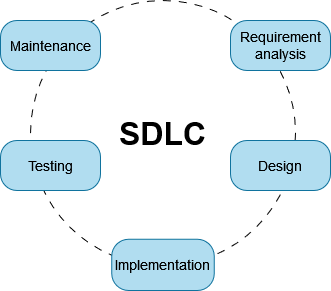
\includegraphics[scale=0.7]{SDLC.png}
    \caption{Software Development Life Cycle}
    \label{fig:sdlc}
\end{figure}

\newpage

\subsection{SDLC Models}

The literature describes several SDLC models that have been used in the development of software applications. \textcite{sdlc1, sdlc2} highlight the most common ones: Waterfall model, V model, Spiral model, Interative model, and Agile model.

\subsubsection{Waterfall Model}

The Waterfall Model is probably the most well-known SDLC model. It is a linear model, where the development process is divided into distinct, sequential phases (which can be seen in figure \ref{fig:waterfall}).

The Waterfall Model's strengths lie in its simplicty of use, ease of understanding and a clear, structured approach \parencite{waterfall}. An additional stregth that the authors note is its extensive documentation and planning, emphasizing quality and adherence to regulations. 

On the other hand, one of Waterfall's main weaknesses is its lack of flexibility in regards to change \parencite{waterfallno}. Thus, this model is not suitable for projects where the requirements are not well understood or are likely to change. Additionally, the project deliverable is not avaialable until the end of the project, any changed or feedback cannot be done during its development \parencite{waterfallno}.

\begin{figure}[ht]
    \centering
    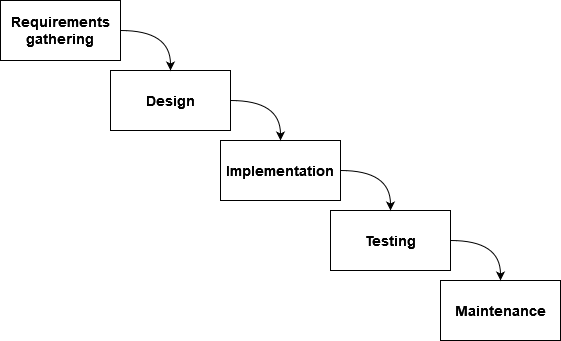
\includegraphics[scale=0.6]{Waterfall.png}
    \caption{Waterfall model}
    \label{fig:waterfall}
\end{figure}

\subsubsection{Agile Model}

Another well-known model is Agile. It has multiple frameworks, with Scrum and Kanban being the most popular ones. Scrum is a framework where the project is divided into sprints, each lasting between 2-4 weeks, that aim on delivering value to the customer through incremental software features \parencite{scrumban, agile}. Kanban focuses on visualizing the project workflow by using a visual board with columns, cards and swimlanes. It uses column limits and a pull system to make the flow of work through the system more efficient \parencite{agile}.

Agile has some drawbacks - its lack of documentation and formal planning, especially in the early stages of the project, may not be suitable for large scale projects \parencite{agile, sdlc2}. Similarly, lack of knowledge on how to use the frameworks may be a barrier for some teams \parencite{waterfallno, sdlc2}.

Nowadays, the combined use of Scrum and Kanban is becoming quite popular, with many teams employing both frameworks in their projects, allowing them to adopt the appropriate practices and adapt them accordingly based on their needs \parencite{scrumban}.

\begin{figure}[ht]
    \centering
    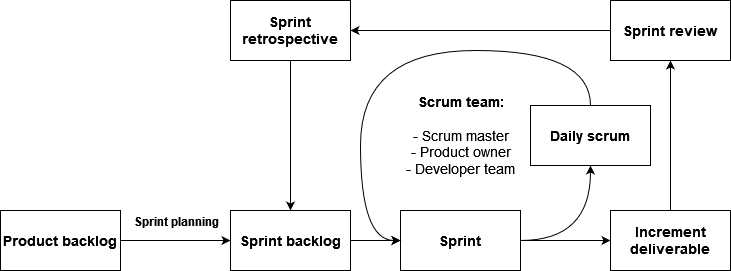
\includegraphics[scale=0.5]{Scrum.png}
    \caption{Scrum framework}
    \label{fig:scrum}
\end{figure}

\subsection{A hybrid approach}

A hybrid approach has also been emerging in software development projects. Various surveys report the most common combinations are Scrum, Iterative Development, Kanban, Waterfall and DevOps, with hybrid Waterfall and Scrum being the most popular one \parencite{hybrid1,hybrid2}. In this approach, the development part is done in an Agile way, with the rest of the project using Waterfall as a backbone \parencite{hybrid2}.

\textcite{hybrid1} note that projects using either Agile, traditional or hybrid approach show similar levels of success in terms of budget, time and quality. However, the authors have found that agile and hybrid approaches perform much better on customer satisfaction than the traditional ones.

\section{Requirements gathering}

Requirements gathering is the first step in any software development process. As described by \textcite{reqanalysis2}, a requirement is a `necessary attribute in a system\ldots that identifies a capability, characteristic, or quality factor of a system in order for it to have value and utility to a user'. Multiple studies mention how proper requirement gathering plays a pivotal role in the project success, with many project failures attributed to poor requirements gathering \parencite{reqanalysis1, reqanalysis3, reqanalysis5}.

\subsection{Requirement types}

Requirements can be classified into 2 categories: functional and non-functional. Functional requirements describe the system's behavior, while non-functional requirements describe the system's quality attributes, such as performance, security, reliability, etc. \parencite[6]{requirements}.

When writing the requirements in a document, it is important to ensure clarity and conciseness to avoid ambiguity. Based on the recommendations of \textcite[112]{requirements} and \textcite{requirements2}, the following principles and practices can be followed:  
\begin{itemize}
    \item Write in a simple and consistent language.
    \item Avoid technical jargon, vague terms, and combining multiple requirements in a single statement.
    \item Ensure that requirements are necessary, appropriate, complete, feasible, and verifiable.
    \item Include attributes for each requirement, such as identification, owner, priority, risk, rationale, difficulty, and type (functional/non-functional).
\end{itemize}

Prioritizing requirements is another crucial task, especially in projects with numerous requirements. Some methods mentioned by \textcite{moscow} include using a low to high priority, assigning a numerical value within a specific range or MoSCoW, which classifies requirements into four categories: 
\begin{itemize}
    \item Must have - must be implemented in the software before being released
    \item Should have - important but not necessary for the software to be released
    \item Could have - desirable but not necessary for the software to be released
    \item Won't have - requirements that are not included in the current release
\end{itemize}

\subsubsection{Requirements in Agile}

In Agile projects, requirements are written in the form of User Stories, which are simple descriptions of a feature desired by the customer, using a specific format: `As a [user], I want to [action] so that [benefit]' \parencite[191]{requirements}. Components of a User Story include a title, acceptance criteria, priority, story points and description. Epics are requirements that cannot be completed in a single sprint and can be broken down into user stories. Epics and User Stories are part of the Product and Sprint backlogs, which contain the requirements for the whole project and the current sprint, respectively.

\subsection{Stakeholders}
\label{sec:stakeholders}

Stakeholders are the individuals who have some interest in the success of the system or project, thus it is important to identify all possible stakeholders in the early stages of the project to avoid missing important requirements or constraints \parencite[34]{requirements}. 

Stakeholder analysis can help understand their position within the project. One way of doing it is by using a stakeholder matrix, such as the Influence/Interest grid (see figure \ref{fig:stakeholder_matrix}), which classifies stakeholders based on their influence and interest in the project \parencite{stakeholders,stakeholders2}.

\begin{figure}[ht]
    \centering
    
\includegraphics[scale=0.5]{Stakeholder.png}
    \caption{Stakeholder Influence/Interest matrix}
    \label{fig:stakeholder_matrix}
\end{figure}

\subsection{Requirement gathering techniques}

Multiple studies mention the most popular requirement gathering techniques are interviews, workshops, prototyping, modelling, brainstorming, storyboards and observing users \parencite{reqanalysis1,reqanalysis2, reqanalysis3, reqanalysis4}. In one of them, individuals with multiple years of experience in requirement gathering were interviewed, and the authors found that the most used techniques were collaborative meetings, interviews, ethnography and modelling \parencite{reqanalysis1}.

Multiple research papers recognise interviews as the most common technique for requirement gathering \parencite{interviews5,interviews1,interviews2}. Some studies have looked at best practices and common mistakes when conducting requirement gathering interviews. The recommended practices, based on \textcite{interviews4, interviews3}, and the common mistakes, from \textcite{interviews1, interviews2}, are summarized in Table \ref{tab:comparison_mistakes_practices} below.

\begin{table}[h!]
    \centering
    \small
    \renewcommand{\arraystretch}{1.2}
    \begin{tabular}{|>{\arraybackslash}m{0.45\textwidth}|>{\arraybackslash}m{0.45\textwidth}|}
    \hline
    \textbf{Common Mistakes} & \textbf{Recommended Practices} \\ \hline
    Wrong opening: failing to understand the context before discussing the problem. & State goals at the beginning and allow customer input at the end. \\ \hline
    Not leveraging ambiguity to reveal knowledge gaps. & Avoid ambiguity by asking clarifying questions. \\ \hline
    Lack of planning: unstructured sequence of questions. & Plan interviews with a structured sequence of questions. \\ \hline
    Failing to build rapport with the customer. & Building rapport through small talk or personal questions in the beginning. \\ \hline
    Implicit goals: failing to ask or clarify stakeholder goals. & Verify alignment and current interpretation with the customer's vision. \\ \hline
    Question omission: not asking about business processes or doing follow-up questions. & Be flexible by probing into relevant topics. \\ \hline
    Weak communication: too much technical jargon usage or not listening to the customer. & Use projective techniques like scenarios to encourage deep thinking. \\ \hline
    Poor question formulation: vague, technical, irrelevant, or too long. & Break down questions or responses into smaller parts and use story telling.  \\ \hline
    Wrong closing sequence: skipping interview summaries or feedback. & Leaving time at the end for the stakeholder to offer any feedback or thoughts. \\ \hline
    \end{tabular}
    \caption{Comparison of Common Mistakes and Recommended Practices}
    \label{tab:comparison_mistakes_practices}
\end{table}

\section{Tech stack}

\subsection{Database}
\label{sec:database}

There are several types of databases, such as: relational (SQL), NoSQL databases, graph databases or object-oriented databases \parencite{databases2}. The choice of database depends on the project or organisation requirements, such as the amount of data, the complexity of the data, the need for scalability, etc. 

\subsubsection{Relational databases}

Relational databases store structured data in tables, linked through keys to create relationships between entries \parencite{databases}. They use SQL (Structured Query Language) to create queries and schemas to help manage data efficiently. \textcite{databases} highlight that relational databases are used, thanks to their high data integrity, for industries like finance and healthcare. Relational databases are widely used, making it easier to find support and resources. However, the rigid schema limits adaptability to rapid data changes or usage of unstructured data. Examples include MySQL, PostgreSQL, Oracle, and Microsoft SQL Server.

\subsubsection{NoSQL databases}

NoSQL databases manage unstructured or semi-structured data without rigid schemas or relationships \parencite{databases}. As the authors describe, NoSQL databases, such as key-value, document, column-family, and graph databases, excel in flexibility and scalability. NoSQL databases often prioritize performance over strict consistency, making them suitable for large datasets of unstructured data but less ideal for complex transactions. NoSQL systems lack SQL’s mature standardization and support. Examples include MongoDB, Cassandra, Couchbase, and Redis.

\subsection{Backend framework}
\label{sec:backend}

Choosing the right backend framework is crucial - it is responsible for handling the business logic of the application, such as processing requests, interacting with the database, and returning responses to the client. A good framework also comes with the added benefit of included features such as security and authentication, database support, a big community and documentation. 

Based on recent a recent survey by \textcite{statista-webframeworks}, the most popular backend frameworks are Express, Flask, Spring Boot, Django and Laravel. This data is also supported by the Stack Overflow Developer Survey 2024, which lists the most popular programming languages as JavaScript (Express), Python (Flask, Django), Java (Spring Boot) and PHP (Laravel) \parencite{stackoverflow}. 

Due to their high popularity among developers, the above frameworks will be compared. Using the information from \textcite{spring,express,django,fastapi}, table \ref{tab:backend} will compare the frameworks based on the following criteria: programming language used, learning curve, community support, security features, database features, and project size suitability.

\begin{table}[h]
    \centering
    \resizebox{\textwidth}{!}{%
    \begin{tabular}{|l|l|l|l|l|}
    \hline
        \textbf{Framework} & \textbf{Django} & \textbf{FastAPI} & \textbf{Spring Boot} & \textbf{Express} \\
    \hline
        \textbf{Language} & Python & Python & Java & JavaScript \\
    \hline
        \textbf{Learning curve} & Medium & Low & High & Low \\
    \hline
        \textbf{Community Support} & High & High & High & High \\
    \hline
        \textbf{Security features} & High & High & High & Medium \\
    \hline
        \textbf{Database features} & Medium & Low & High & Medium \\
    \hline
        \textbf{Project size suitability} & Small to medium & Small to medium & Medium to large & Small to medium \\
    \hline
    \end{tabular}%
    }
    \caption{Comparison of backend frameworks}
    \label{tab:backend}
\end{table}

\subsection{Frontend framework}
\label{sec:frontend}

Similar to the backend frameworks, choosing a suitable frontend framework is equally important - it is responsible for the user interface of the application, such as displaying data, handling user interactions, and making requests to the backend. 

Based on the same survey by \textcite{statista-webframeworks}, the most popular frontend frameworks are React, Angular, Vue.js, and Svelte. This data is also supported by the Stack Overflow Developer Survey 2024, where those frameworks rank among the highest for desirability and admirability among developers \parencite{stackoverflow}.

Table \ref{tab:frontend} will use the information from \textcite{react,angular,vue,svelte} to compare the frameworks based on the following criteria: learning curve, community and documentation, ecosystem and tooling support, performance, state management, and project size suitability.

\begin{table}[h]
    \centering
    \resizebox{\textwidth}{!}{%
    \begin{tabular}{|l|l|l|l|l|}
    \hline
        \textbf{Framework} & \textbf{React} & \textbf{Angular} & \textbf{Vue.js} & \textbf{Svelte} \\ 
    \hline 
        \textbf{Learning curve} & Low & High & Medium & Low \\ 
    \hline
        \textbf{Community and documentation} & High & High & High & Medium \\ 
    \hline
        \textbf{Ecosystem and tooling support} & High & High & Medium & Low \\ 
    \hline
        \textbf{Performance} & High & Medium & Medium & High \\ 
    \hline
        \textbf{State management} & High & High & Medium & Low \\ 
    \hline
        \textbf{Project size suitability} & Small to large & Medium to large & Small to medium & Small to medium \\ 
    \hline
    \end{tabular}%
    }
    \caption{Comparison of frontend frameworks}
    \label{tab:frontend}
\end{table}

\section{Large Language Models (LLMs)}

Large language models (LLMs) are artificial intelligence systems that are used for natural language processing (NLP) tasks such as text generation, translation, summarization and question answering \parencite{llm2,llm_healthcare}. Additionally, LLMs have been found to have emergent capabilities, like reasoning, planning, decision-making and in-contenxt learning \parencite{llm2}. These extraordinary capabilities are achieved through extensive training on large corpus of text data, high parameter count (in the billions) and usage of techniques such as fine-tuning or prompt engineering to improve their performance \parencite{llm2,llm_healthcare}.

LLMs are built on the transformer architecture, which allows them to understand text by learning and remembering the relationships between words \parencite{llm}. These models are first pre-trained on large amounts of unlabeled data using, allowing them to excel in a wide variety of tasks \parencite{foundation, llm2}. These pre-trained models, known as foundation models such as the GPT or Llama families, can then be fine-tuned for specific tasks, improving their performance and accuracy even further \parencite{gpt4,llama3,llm2}.

\subsection{Multimodal LLMs}

One advancement in the field of LLMs has been the addition of multimodal abilities, allowing them to process, understand and generate text and images, audio or videos \parencite{mllm, mllm2}. These new multimodal LLMs (MLLMs) utilise existing reasoning capabilities of LLMs, which are connected to an encoder that can processes images, audio or videos and a generator that helps with generating multimodal outputs \parencite{mllm}. This integration of new modalities allows MLLMs to become versatile tools, expanding their possible use cases and bridging the gap between human and machine interaction \parencite{llm_healthcare}.

\subsubsection{API model providers}

Running and hosting LLMs locally can be a challenge, considering their big model sizes and high computational requirements. As such, many platforms offer APIs that allow users to access LLMs through the cloud. A list of some free API providers, the models offered and their rate limits has been compiled by \textcite{llmapi} and some are listed in the table below.

\begin{table}[h!]
    \centering
    \begin{tabular}{p{2cm} p{5cm} p{6cm}}
        \toprule
        \textbf{Provider} & \textbf{Model name(s)} & \textbf{Free tier limits} \\
        \midrule
        \raggedright
        Groq & Llama 3.2 11B Vision & 7,000 requests/day, 7,000 tokens/minute \\
        & Llama 3.2 90B Vision & 3,500 requests/day, 7,000 tokens/minute \\
        \hline
        \raggedright
        OpenRouter & Llama 3.2 11B Vision Instruct &  \\
        & Llama 3.2 90B Vision Instruct & 20 requests/minute, 200 requests/day \\
        & Gemini 2.0 Flash Experimental &  \\
        \hline
        \raggedright
        Google AI Studio & Gemini 2.0 Flash & 4,000,000 tokens/minute, 10 requests/minute \\
        & Gemini 1.5 Flash & 1,000,000 tokens/minute, 1,500 requests/day, 15 requests/minute \\
        & Gemini 1.5 Pro & 32,000 tokens/minute, 50 requests/day, 2 requests/minute \\
        \hline
        \raggedright
        GitHub Models & OpenAI GPT-4o & Rate limits dependent on Copilot subscription tier \\
        & OpenAI GPT-4o mini & \\
        \hline
        \raggedright
        Cloudflare Workers AI & Llama 3.2 11B Vision Instruct & 10,000 tokens/day \\
        \hline
        \raggedright
        glhf.chat & Any model on Hugging Face that fits on an A100 node (~640GB VRAM)& 480 requests/8 hours \\
        \bottomrule
    \end{tabular}
    \caption{API providers for LLMs}
    \label{tab:llm_apis}
\end{table}

\FloatBarrier
\clearpage

\subsection{LLMs in healthcare}

One application of MLLMs is in healthcare, where the growing volume and complexity of data creates the need for more advanced tools to process and analyze it. LLMs and MLLMs have found use in various healthcare applications, either by using existing models or by developing new, specialized medical models such as Med-PaLm2, BioMistral or Med-Gemini \parencite{biomistral,medgemini,medpalm2}. Some of these applications include:

\begin{itemize}
    \item \textbf{Improving medical diagnosis:} By combining patient records, existing symptoms, and medical history, LLMs can use their reasoning capabilities and memory to assist in diagnosing or preventing health conditions \parencite{llm_healthcare,llm_healthcare3,llm_healthcare4}.
    \item \textbf{Medical Imaging and Multimodal Capabilities:} In diagnostic imaging, multimodal models can assess both text and images (such as X-rays and MRIs) to offer comprehensive analysis. Clinicians can input medical images and contextual information, making MLLMs valuable assistants in the real-time diagnostic processes \parencite{llm_healthcare3}.
    \item \textbf{Virtual Health Assistants:} LLMs can also be deployed as virtual assistants, helping patients with personalised care and general health inquiries \parencite{llm_healthcare,llm_healthcare3}. Patients in areas with limited healthcare access can benefit from these assistants, which also supports healthcare providers by lightening their workloads.
    \item \textbf{Administrative Support:} LLMs can assist in generating Electronic Health Records (EHRs), allowing healthcare providers to focus more on patient interaction \parencite{llm_healthcare4}. Additionally, they can also help translate complex medical terms into more simple language, assist in administrative tasks, and more.
\end{itemize}

\subsection{Prompt Engineering}

The success of LLMs depends not only on the model itself - but also on how it's effectively used by the users, using techniques like prompt engineering, which involves the constant designing and refining of prompts to guide the output of LLMs \parencite{promptmed,prompt2}. Prompts represent instructions given to the model to guide its output, such as providing context, examples, or constraints to the model \parencite{prompt,prompt1,prompt2}. 

There are multiple techniques for prompt engineering, ranging from simple to more advanced. The tables and subsections below outlines some of the most common techniques.

\subsubsection{Zero-Shot Prompting}

Zero-shot prompting are techniques where the LLM is given a prompt without any examples, allowing it to generate an output based on the prompt alone \parencite{prompt1}.

\begin{table}[h!]
    \centering
    \begin{tabular}{p{3cm} p{8cm} p{2cm}}
        \toprule
        \textbf{Technique} & \textbf{Description} & \textbf{Source} \\
        \midrule
        \raggedright
        Role prompting & Assigning a specific role to the LLM in the prompt. The authors note that generally it provides mixed results but may be useful in certain settings.  & \textcite{role1} \\
        \hline
        \raggedright
        Style prompting & Specifying the desired style or tone in the prompt. & \textcite{style} \\
        \hline
        \raggedright
        Emotion prompting & Incorporating phrases of psychological relevance to humans in the prompt. & \textcite{emotion} \\
        \hline
        \raggedright
        Re-reading & Adding the phrase `Read the question again' to the prompt in addition to repeating the question. & \textcite{rereading} \\
        \hline
        \raggedright
        Self-Ask & Prompting the LLM to decide if it needs to ask any follow-up questions for a given prompt. &  \textcite{selfask} \\
        \bottomrule
    \end{tabular}
    \caption{Zero-Shot Prompt Techniques}
    \label{tab:zero_shot}
\end{table}

\FloatBarrier

\subsubsection{Few-Shot Prompting}

Few-shot prompting are techniques where the LLM learns how to complete a task based on a few examples given in the input prompt \parencite{prompt1}.

\begin{table}[h!]
    \centering
    \begin{tabular}{p{3cm} p{8cm} p{2cm}}
        \toprule
        \textbf{Technique} & \textbf{Description} & \textbf{Source} \\
        \midrule
        \raggedright
        Self-Generated In-Context Learning & Using the LLM to automatically generate examples when training/example data is not avaialable. & \textcite{self-generating} \\
        \hline
        \raggedright
        Prompt Mining & Scanning the training data to discover common formats that can be used as prompt templates. & \textcite{mining} \\
        \bottomrule
    \end{tabular}
    \caption{Few-Shot Prompt Techniques}
    \label{tab:few_shot}
\end{table}

\FloatBarrier

\subsubsection{Thought Generation Prompting}

Thought generation are techniques where the prompt encourages the LLM to explain its reasoning process while solving a given problem \parencite{prompt1}.

\begin{table}[h!]
    \centering
    \begin{tabular}{p{3cm} p{8cm} p{2cm}}
        \toprule
        \textbf{Technique} & \textbf{Description} & \textbf{Source} \\
        \midrule
        \raggedright
        Chain-of-Thought (CoT) & Adding a phrase like `Let's think step by step' at the end of the prompt to encourage the LLM to describe its thought process before offering a final answer. & \textcite{cot} \\
        \hline
        \raggedright
        Contrastive CoT & Using CoT and also adding both incorrect and correct examples in order to provide the LLM a more diverse example set.  & \textcite{contrastive-cot} \\
        \hline
        \raggedright
        Auto-CoT & Using CoT with another LLM to automatically generate CoT examples that can be used to create few-shot CoT prompts for other LLMs. &  \textcite{auto-cot} \\
        \hline
        \raggedright
        Least-to-Most & Starts with asking the model to break down a problem into sub-problems without solving them. Afterwards, it solves them one by one, appending the result each time, until it arrives at the answer. & \textcite{least-most} \\
        \hline
        \raggedright
        Tree-of-Thought (ToT) & Starts with an initial problem and then generates multiple possible steps by using CoT. Then, it evaluates each step, decides which one to take and creates more thoughts until it reaches an answer. & \textcite{treeofthought} \\
        \bottomrule
    \end{tabular}
    \caption{Thought Generation Prompt Techniques}
    \label{tab:thought_gen}
\end{table}

\FloatBarrier

\subsubsection{Multimodal and Multilingual Prompting}

Multimodal and multilingual prompting are techniques which aim to improve an LLM's performance by leveraging multiple modalities or languages in the prompt \parencite{prompt1}.

\begin{table}[h!]
    \centering
    \begin{tabular}{p{3cm} p{8cm} p{2cm}}
        \toprule
        \textbf{Technique} & \textbf{Description} & \textbf{Source} \\
        \midrule
        \raggedright
        Translate-first prompting & Translating the input prompt into English to leverage LLMs strengths in dealing with English inputs, compared to non-English inputs. & \textcite{translate-first} \\
        \hline
        \raggedright
        English prompting & Writing the prompt in English may usually be more effective than using the task language for multilingual tasks. The authors argue it may because of the predominance of the English language in the pre-training data. & \textcite{english-prompting} \\
        \hline
        \raggedright
        JSON/XML output formatting & Asking the LLM to format the response in a JSON or XML format and providing the expected schema has been found to improve the accuracy of LLM outputs  & \textcite{jsonllm} \\
        \hline
        \raggedright
        Multimodal CoT & Similar to the textual CoT, this technique encourages the model to solve a given image-based problem step by step by step. & \textcite{multimodal-cot} \\
        \hline
        \raggedright
        Image-as-Text & Generating or writing a textual description of an image that can then be included in a text-based prompt. & \textcite{images-as-text} \\
        \hline
        \raggedright
        Chain-of-Images (CoI) & Using the CoT process to generate images as part of its thought process to reason visually. & \textcite{coi} \\
        \bottomrule
    \end{tabular}
    \caption{Multimodal and Multilingual Techniques}
    \label{tab:multi_prompt}
\end{table}

\FloatBarrier

\subsubsection{Agents}

Agents are techniques which encourage LLMs to use external tools or resources to complete a task \parencite{prompt1}.

\begin{table}[h!]
    \centering
    \begin{tabular}{p{3cm} p{8cm} p{2cm}}
        \toprule
        \textbf{Technique} & \textbf{Description} & \textbf{Source} \\
        \midrule
        \raggedright
        Program-aided Language Model (PAL) & Using the LLM to translate a problem into code, which can then be sent to an interpreter to generate an answer. & \textcite{pal} \\
        \hline
        \raggedright
        ReAct & Firstly, the model generates a thought based on the input. Then, the model takes an action and observes the result. This process is repeated until the model arrives at an answer. & \textcite{react-llm} \\
        \hline
        \raggedright
        Retrieval Augmented Generation (RAG) & This technique involves retrieval of information from an external source and inserting it into the prompt. & \textcite{rag} \\
        \bottomrule
    \end{tabular}
    \caption{LLM Agent Techniques}
    \label{tab:agents}
\end{table}

\FloatBarrier

\subsection{Challenges and concerns of using LLMs}

While LLMs bring many benefits when applied to the healthcare domain, it is important to note that their use does come with several challenges:

\begin{itemize}
    \item \textbf{Data Privacy and Compliance:} Patient data is highly sensitive, thus ensuring compliance with standards is essential, requiring data anonymization and secure handling practices to ensure patient data safety.\parencite{llm_healthcare,llm_healthcare2,llm_healthcare4}.
    \item \textbf{Transparency and Explainability:} LLMs are often described as `black boxes', making it difficult to explain their decision-making processes. In healthcare, transparency is crucial - lack of it poses risks and raises ethical concerns about relying on such systems in high-stakes scenarios \parencite{llm_healthcare,llm_healthcare2,llm_healthcare4}..
    \item \textbf{Bias and Fairness:} LLMs trained on vast datasets can inherit biases in the data, leading to skewed or unfair outcomes \parencite{llm_healthcare2}.
    \item \textbf{Hallucinations:} LLMs sometimes generate false or fabricated outputs, also known as `hallucinations'. In healthcare, this poses significant risks, as incorrect or misleading information could jeopardize patient safety and trust in the technology \parencite{llm_healthcare4,llm_healthcare}.
    \item \textbf{Accountability:} Responsibility must be clearly communicated and understood by all parties involved in the development and use of the model \parencite{llm_healthcare2}. The author recommends the usage of clear guidelines, policies and code of conducts to ensure that all parties are aware of their obligations.
    \item \textbf{High Costs and Infrastructure Needs:} Training and operating LLMs requires extensive computational resources, which can be a limiting factor for healthcare institutions \parencite{llm_healthcare4}.
\end{itemize}

\section{PHR Systems}

A Personal Health Record (PHR) is an electronic resource
used by patients to manage their own health information \parencite{phrsecurity,phrlist}. PHRs are different from Electronic Health Records (EHRs) and Electronic Medical Records (EMRs) which are inter-organisational or internal systems to organise patient health records \parencite{phrdiff,phrlist}. Three different types of PHRs are described by \textcite{phrsecurity}: stand-alone, which require manual entry to update the records; instituion-specific, which are connected to a specific healthcare institution; and integrated, which can connect to multiple healthcare systems to aggregate data from multiple sources. 

Usage of PHRs can bring many benefits to patients, such as: empowering patients to manage their health, improving patient outcomes, decreasing the cost of healthcare and improving the taking of medication \parencite{phrsecurity}.

PHRs contain highly sensitive health information, so it is important to ensure that the data is secure and private. Based on a survey of health information management and medical informatics experts, \textcite{phrsecurity} identified 7 dimensions that need to be addressed when developing a PHR system:
\begin{enumerate}
    \item Confidentiality
    \item Availability
    \item Integrity
    \item Authentication
    \item Authorization
    \item Non-repudiation
    \item Access rights
\end{enumerate}

The authors recommend mechanisms to ensure adherence to the above-mentioned dimensions, such as encrypting the data in the database, using backups or defining user access to data and access rights.

\subsection{Existing Solutions}

PHR systems have been implemented nation-wide in many developed countries, such as the NHS App in the UK \parencite{phrlist}. Additionally, there are many private solutions that offer similar features to the one proposed in this project. The next sections will provide a brief overview of 3 existing systems: Medvalet, Andaman7 and Fasten Health.

\subsubsection{Medvalet}

A mobile app developed in Romania that allows patients to upload their medical history as PDFs or scanned documents \parencite{medvalet}. See Table \ref{tab:medvalet} for a summary of its features and limitations and figure \ref{fig:medvalet} for a screenshot of the app.

\begin{figure}[h!]
    \centering
    \subfloat[My doctors screen]{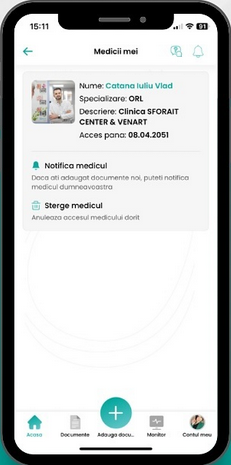
\includegraphics[width=0.35\textwidth]{Medvalet_1.png}} \quad
    \subfloat[Uploaded documents screen]{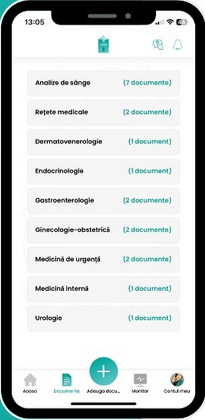
\includegraphics[width=0.35\textwidth]{Medvalet_2.png}}
    \caption{Medvalet screenshots}
    \label{fig:medvalet}
\end{figure}

\begin{table}[h!]
\centering
    \begin{tabular}{|p{0.47\textwidth}|p{0.47\textwidth}|}
    \hline
    \textbf{Key Features/Benefits} & \textbf{Limitations/Drawbacks} \\ \hline
    \begin{itemize}
        \item Upload medical history as PDFs or scanned documents.
        \item Categorize documents by type (e.g., prescriptions, lab results).
        \item Graphically track vitals like blood pressure and weight over time.
        \item Patients can input personal details such as name, age, and weight.
        \item Doctors can access patient history directly via the app.
    \end{itemize} &
    \begin{itemize}
        \item Requires doctors to create accounts, which may deter use.
        \item Doctors can access patient history without explicit consent, raising privacy concerns.
        \item App acts as document storage, which can be cumbersome to access for lengthy histories.
        \item Lacks data extraction or summarization features from uploaded documents.
        \item Only available as a mobile app, limiting accessibility for desktop-only users.
    \end{itemize} \\ \hline
    \end{tabular}
\caption{Medvalet Features and Limitations}
\label{tab:medvalet}
\end{table}

\FloatBarrier

\subsubsection{Andaman7}

A mobile app developed by a Belgian-American eHealth company with the goal to improve doctor-patient communication, compliant with GDPR and HIPAA \parencite{andaman}. See Table \ref{tab:andaman7} for a summary of its features and limitations and figure \ref{fig:andaman7} for a screenshot of the app.

\begin{figure}[ht]
    \centering
    \subfloat[PHR Sections screen]{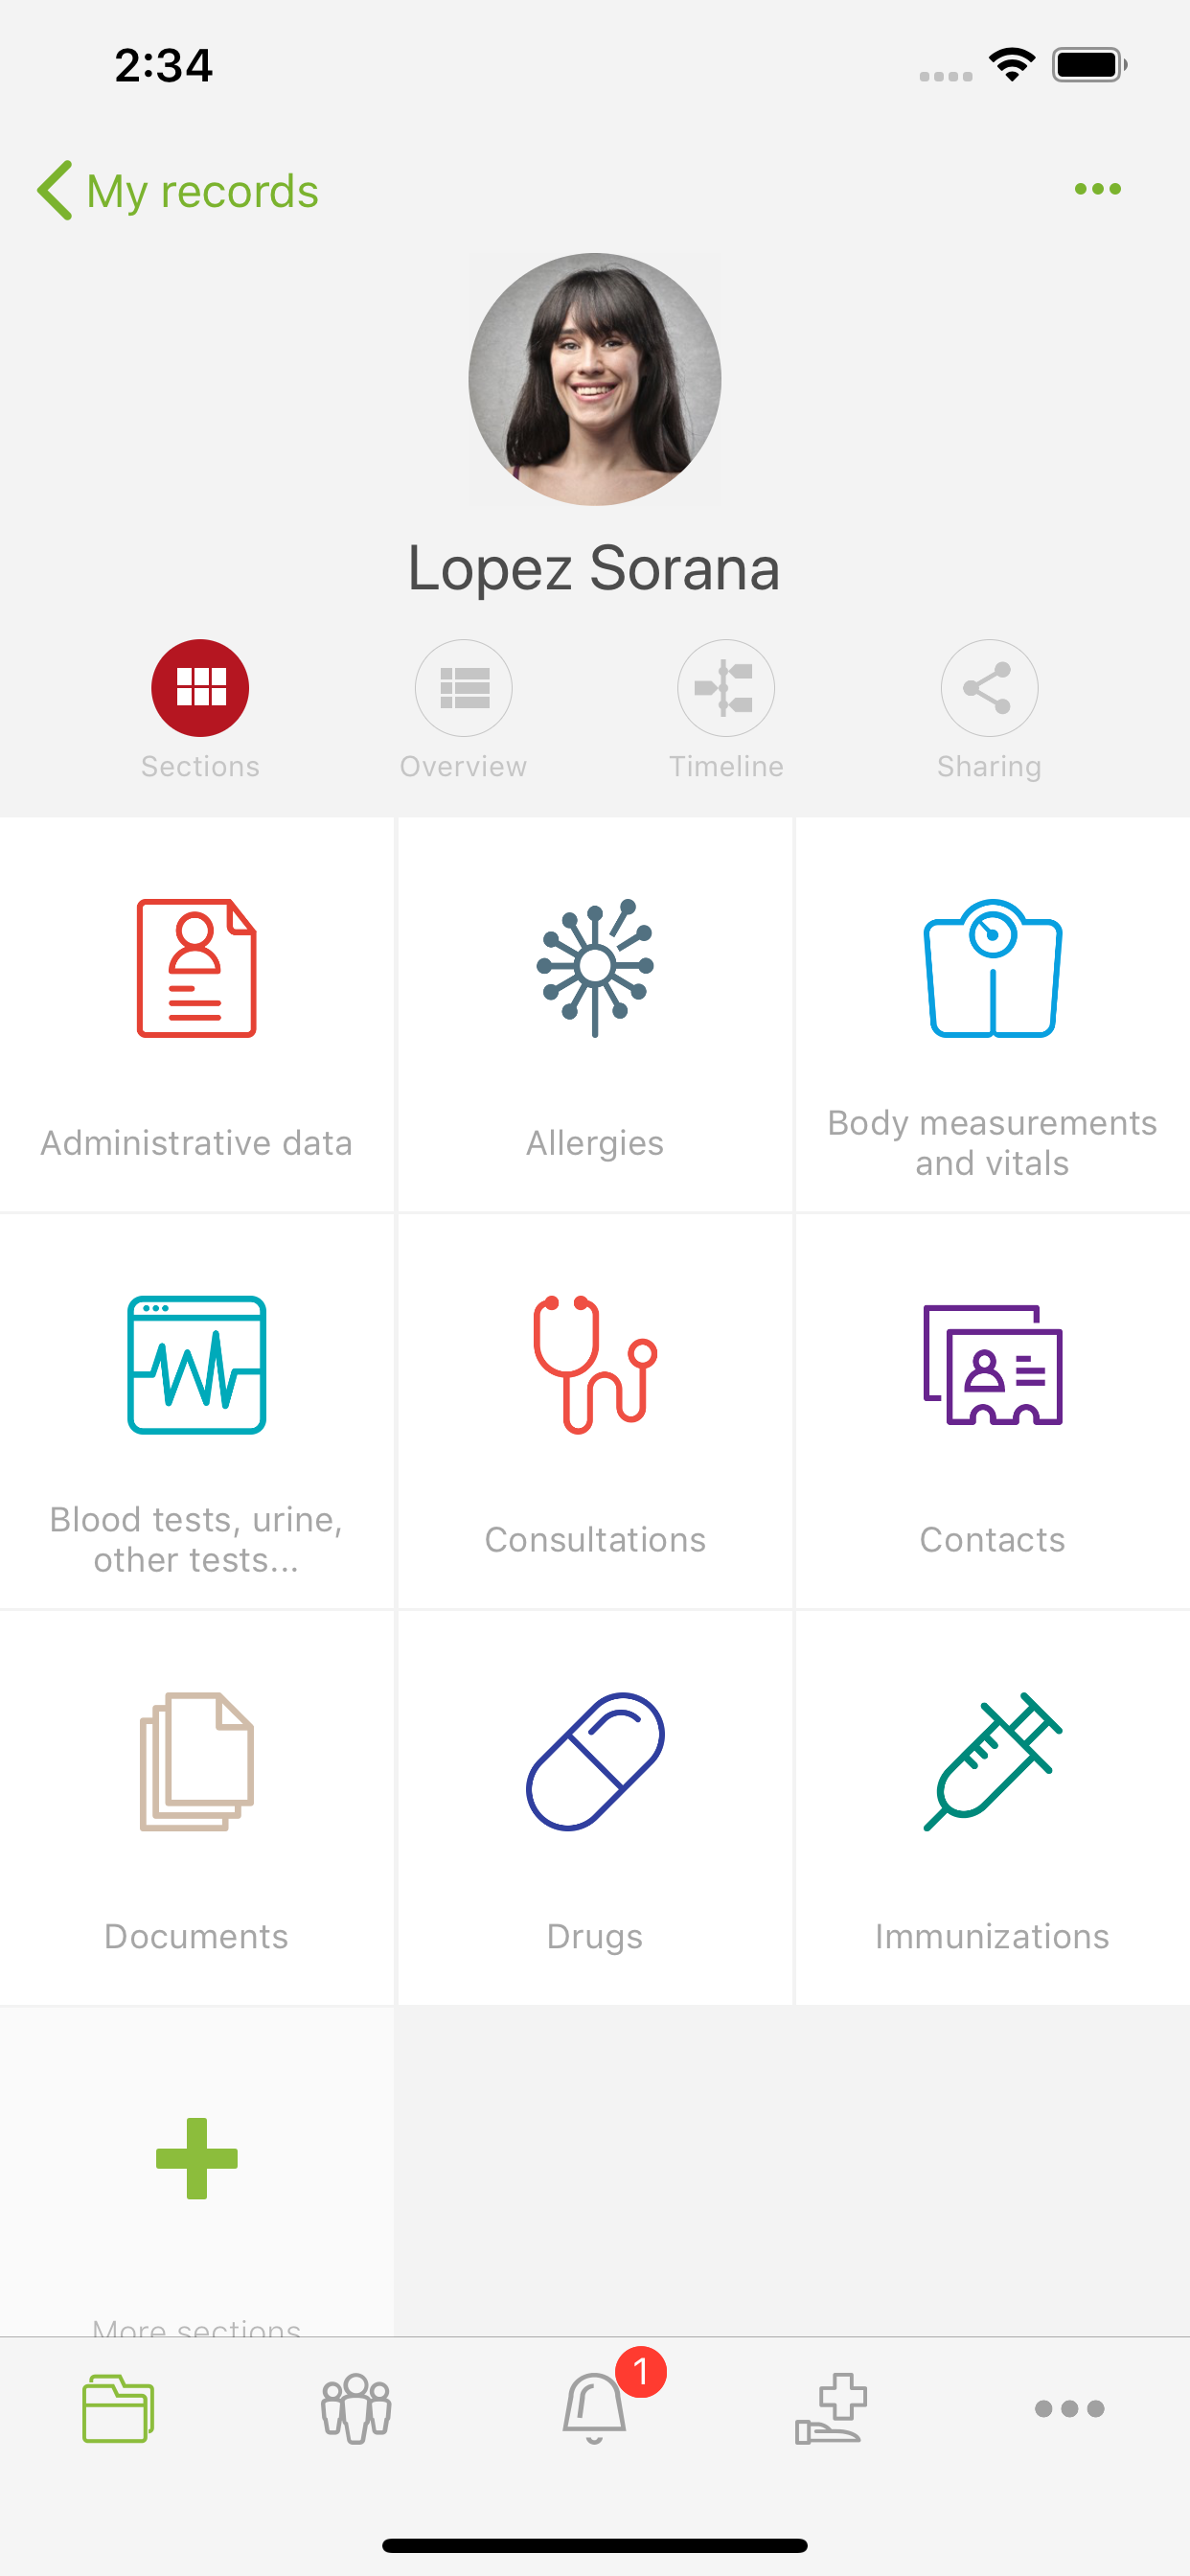
\includegraphics[width=0.45\textwidth]{Andaman_1.png}} \quad
    \subfloat[Documents section screen]{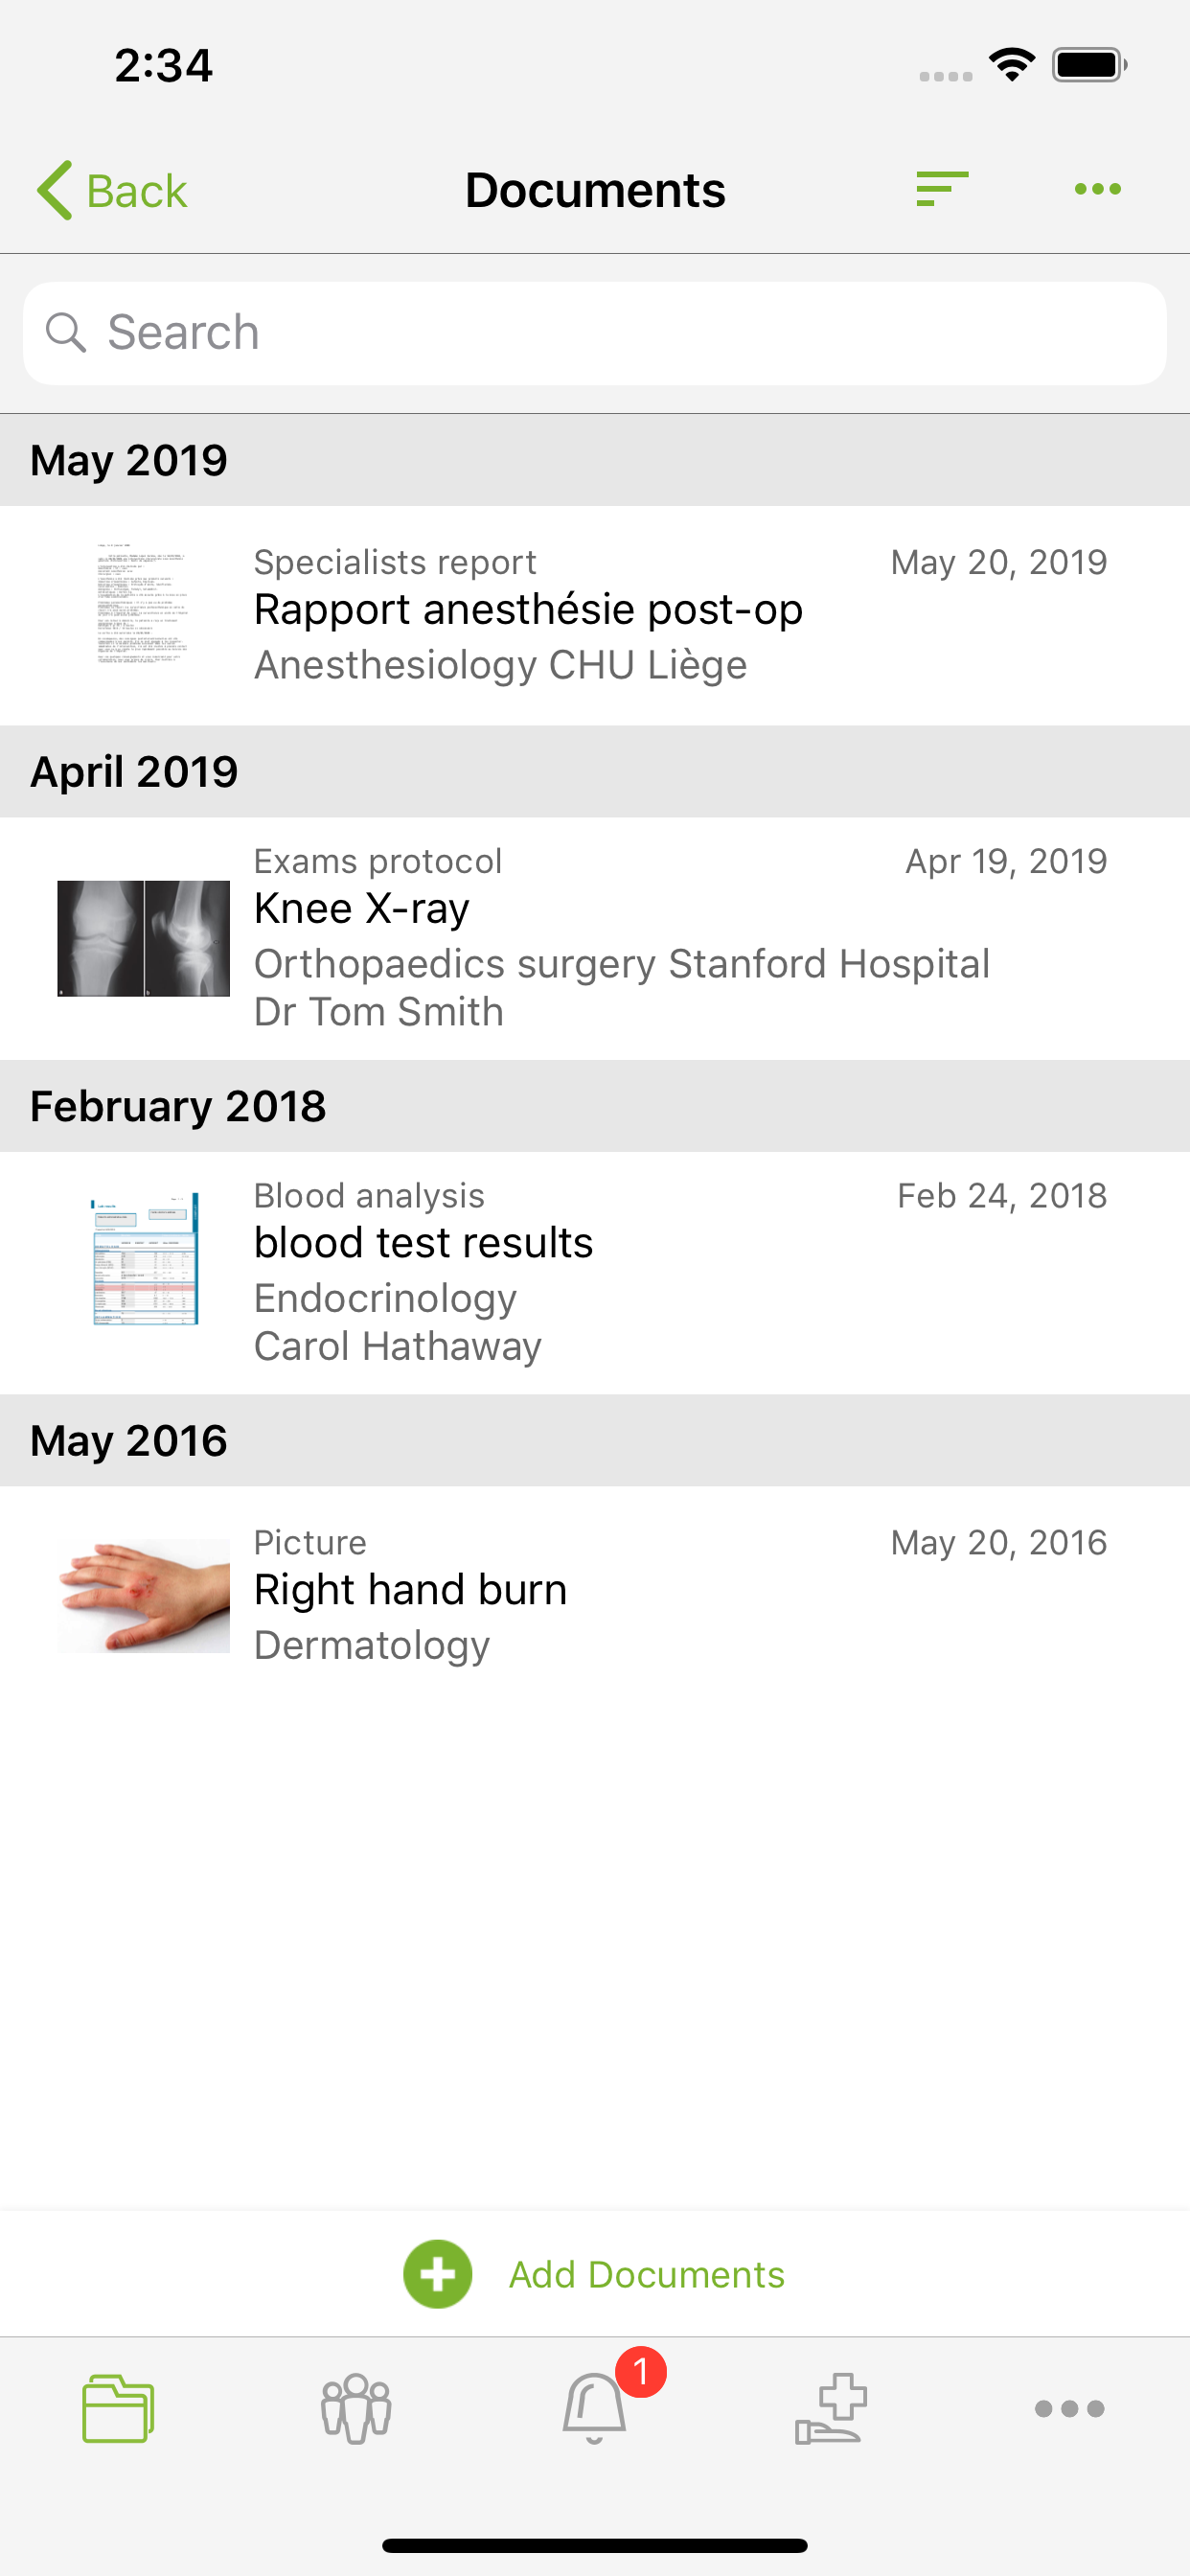
\includegraphics[width=0.45\textwidth]{Andaman_2.png}}
    \caption{Andaman7 screenshots}
    \label{fig:andaman7}
\end{figure}

\begin{table}[htbp]
\centering
    \begin{tabular}{|p{0.47\textwidth}|p{0.47\textwidth}|}
    \hline
    \textbf{Key Features/Benefits} & \textbf{Limitations/Drawbacks} \\ \hline
    \begin{itemize}
        \item Offers sections for personal information, medical history, allergies, vaccinations, medications, etc.
        \item Automatically collects health data from over 300 hospitals and clinics in the US and Europe.
        \item Supports input from diverse sources like hospitals, labs, smart devices or even manual input.
        \item Stores data locally on patients’ devices, ensuring privacy.
        \item Data sharing with QR codes and revokable access.
        \item AI tools for summarization, translation, and simplifying medical jargon.
    \end{itemize} &
    \begin{itemize}
        \item Requires patients and doctors to both create accounts.
        \item Does not extract data or values from uploaded documents like lab results.
        \item Limited to mobile platforms, which may limit usability for desktop-only users.
    \end{itemize} \\ \hline
    \end{tabular}
\caption{Andaman7 Features and Limitations}
\label{tab:andaman7}
\end{table}

\FloatBarrier

\subsubsection{Fasten Health}

An open-source, self-hosted electronic medical record aggregator with optional paid desktop versions for Windows and Mac \parencite{fasten}. See Table \ref{tab:fasten_health} for a summary of its features and limitations and figure \ref{fig:fasten} for a screenshot of the app.

\begin{figure}[ht]
    \centering
    \subfloat[Dashboard screen]{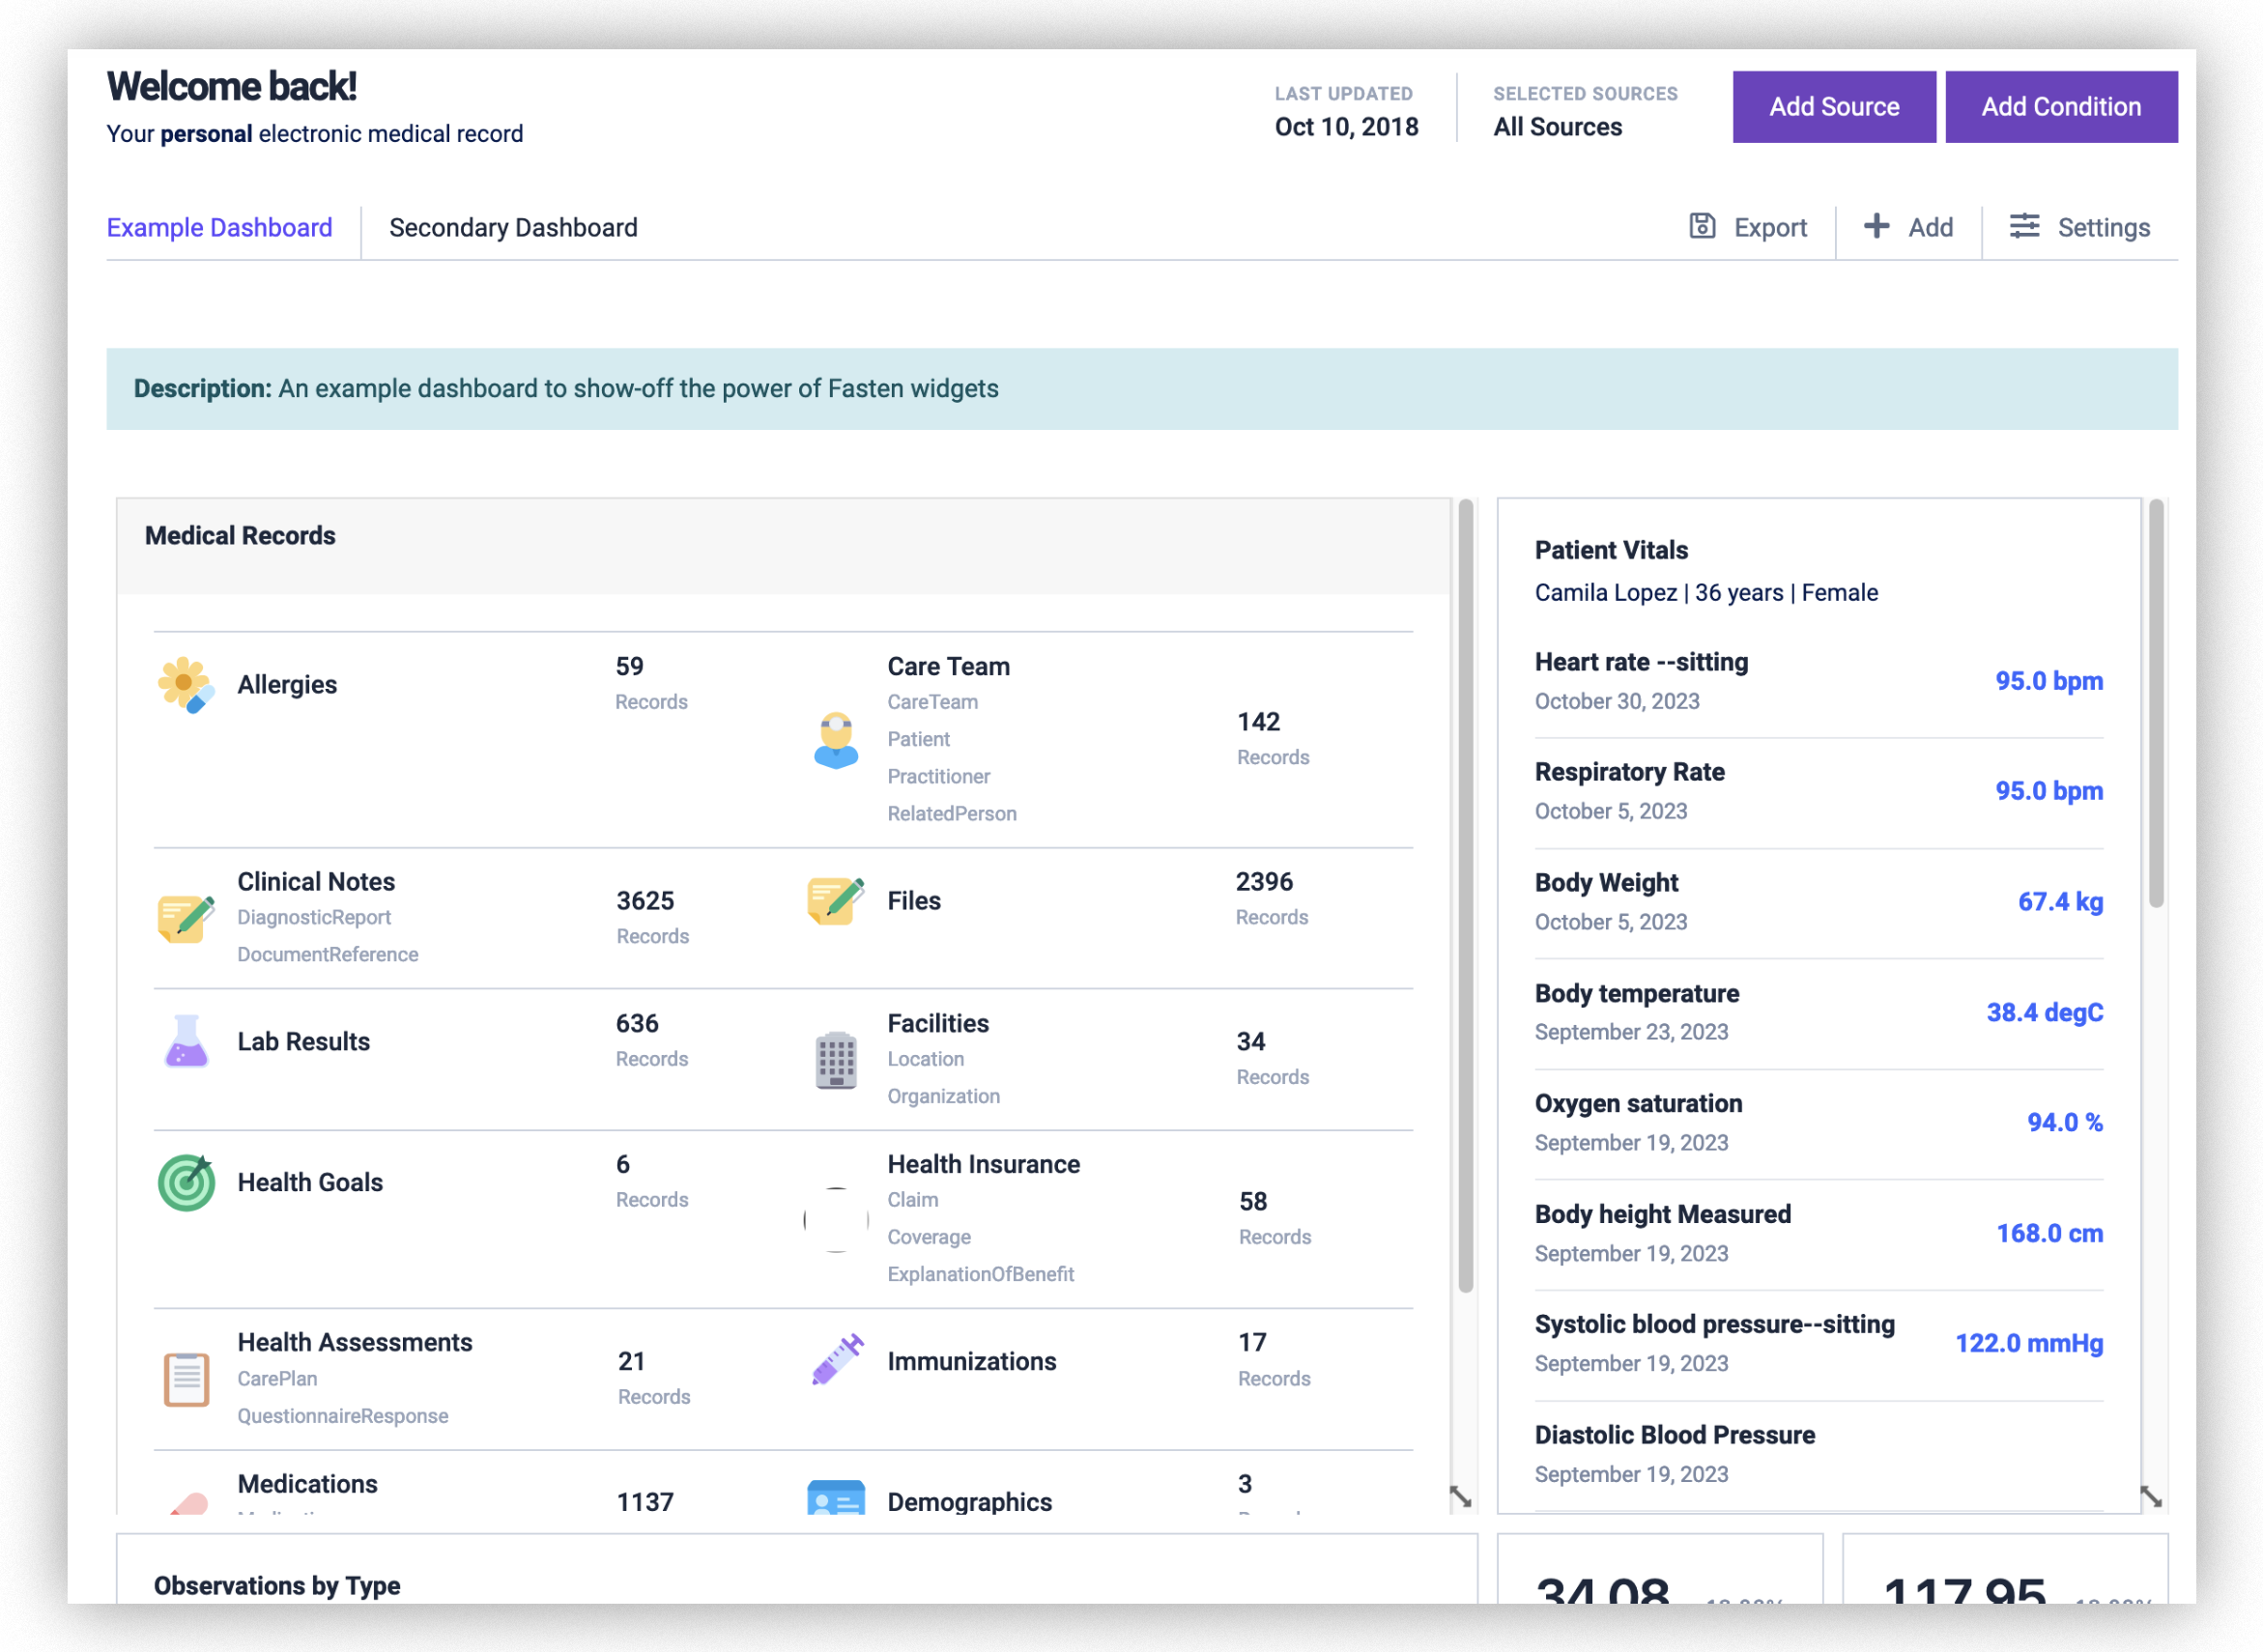
\includegraphics[width=0.75\textwidth]{fasten_1.png}\label{fig:fasten1}} 
    \hspace{0.05\textwidth} 
    \subfloat[Visit history screen]{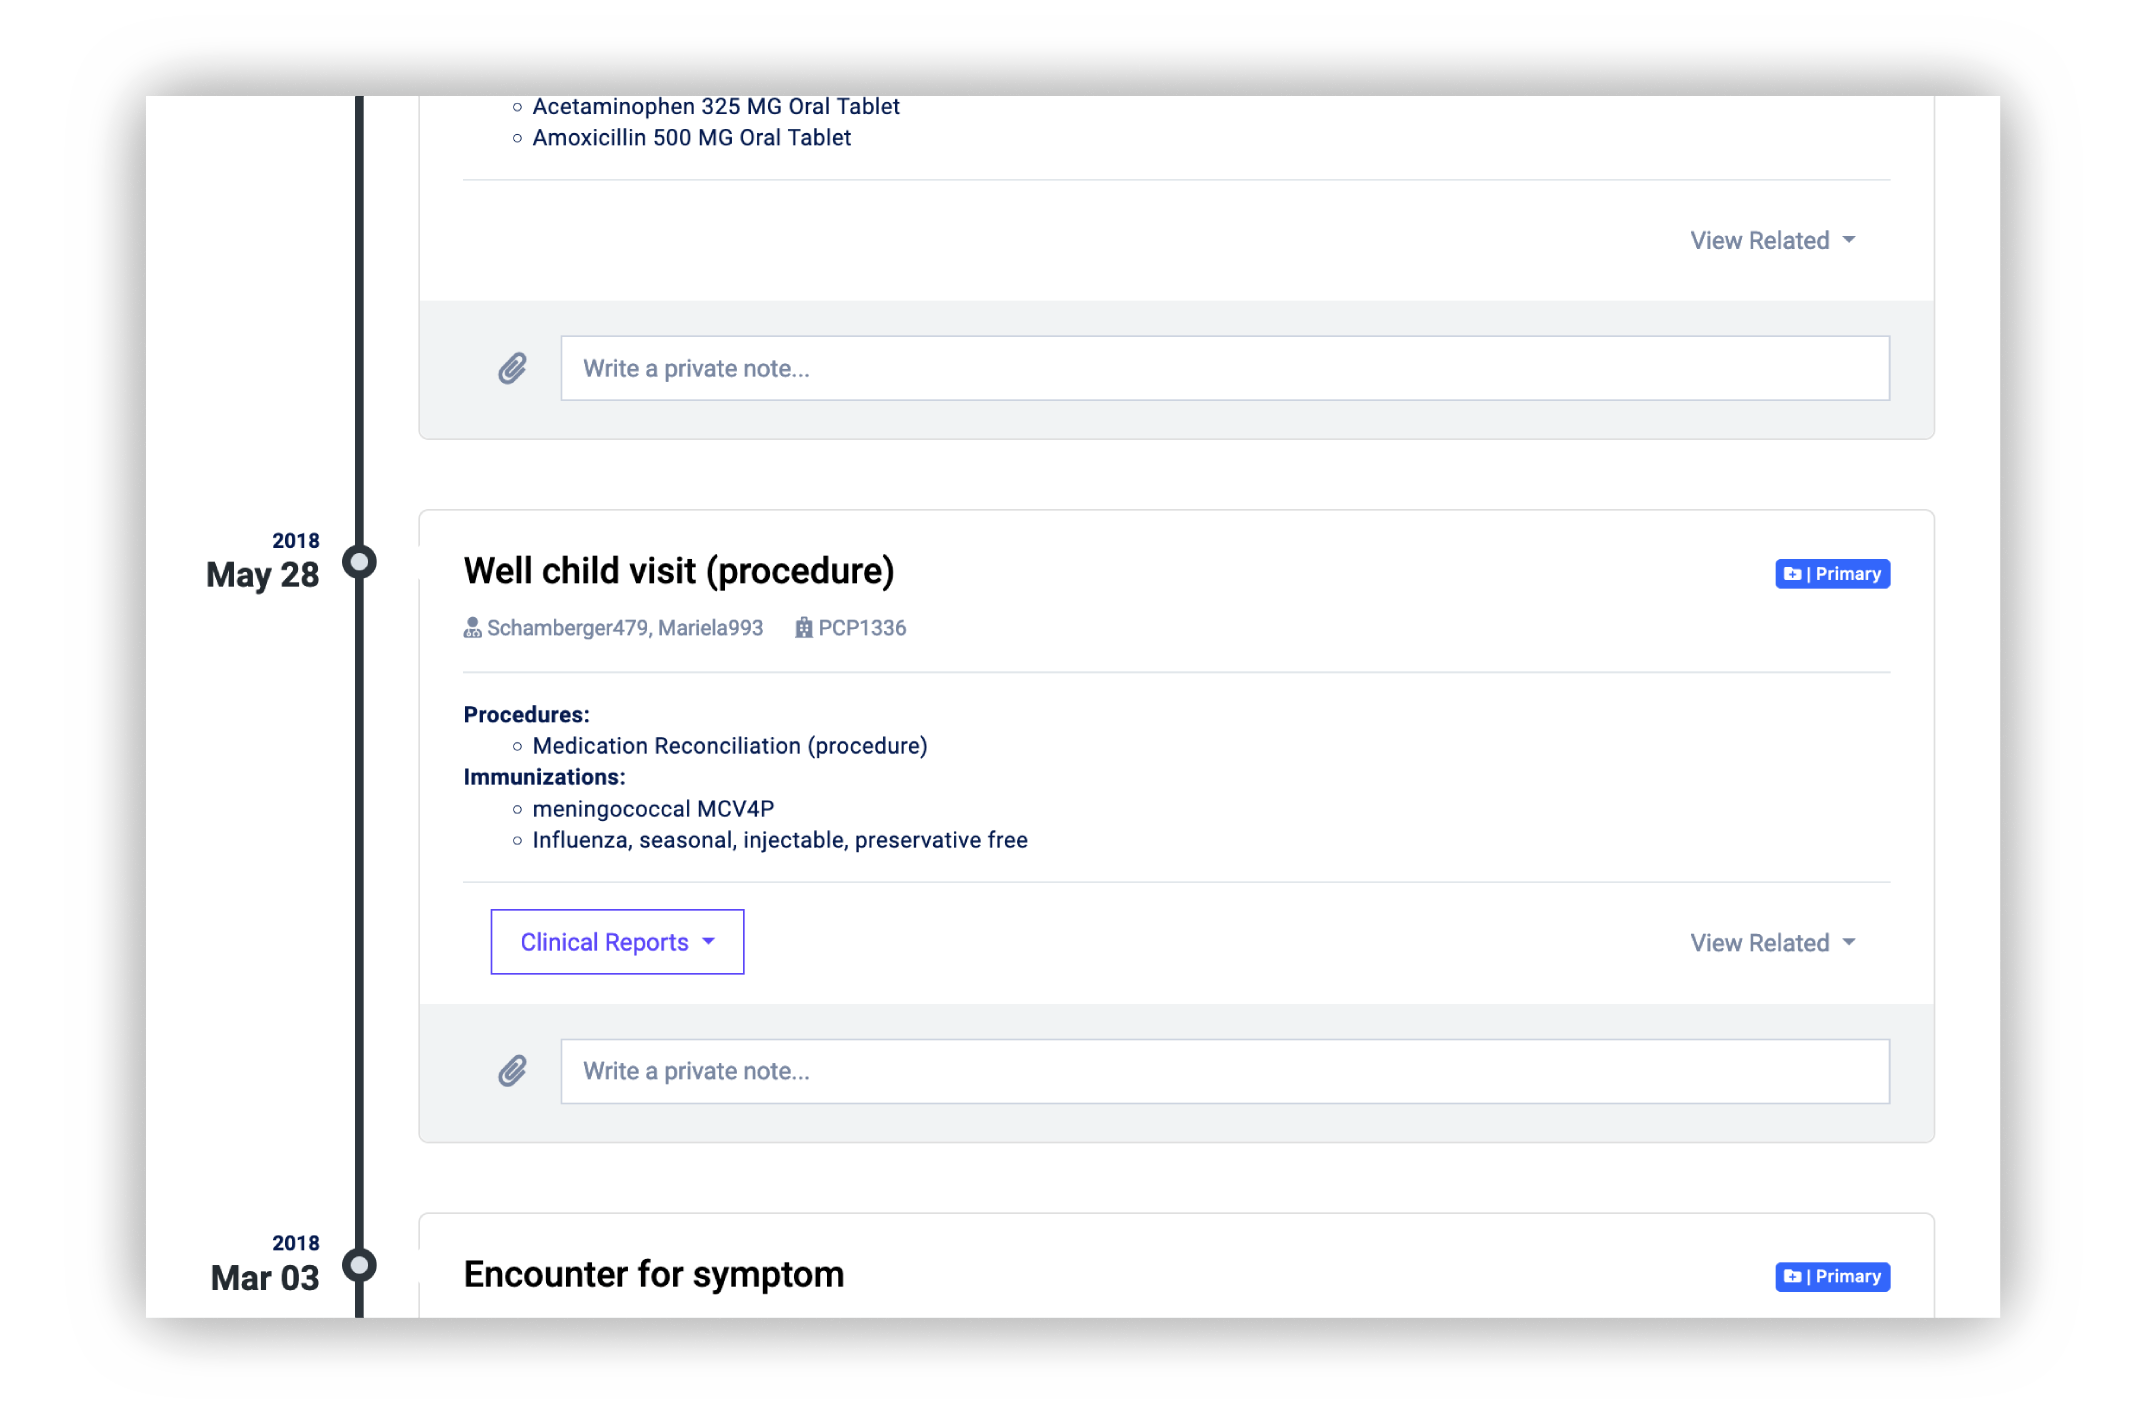
\includegraphics[scale=0.3]{fasten_2.png}\label{fig:fasten2}} 
    \caption{Fasten Health screenshots}
    \label{fig:fasten}
\end{figure}

\begin{table}[h!]
\centering
    \begin{tabular}{|p{0.47\textwidth}|p{0.47\textwidth}|}
    \hline
    \textbf{Key Features/Benefits} & \textbf{Limitations/Drawbacks} \\ \hline
    \begin{itemize}
        \item Automatically aggregates records from multiple providers, like hospitals and labs.
        \item Supports self-hosting for complete control over data, stored locally.
        \item Compatible with protocols such as DICOM, FHIR, and OAuth2.
        \item Allows manual entry for allergies, vaccinations, and medications.
        \item Offers multiple dashboards with graphs to visualize health data.
        \item Supports multi-user functionality for families.
    \end{itemize} &
    \begin{itemize}
        \item Paid desktop versions may deter users.
        \item Manual data entry limited to new or existing encounters, complicating usage.
        \item Does not support OCR or automatic data extraction from documents.
        \item Lacks data-sharing capabilities with doctors.
        \item Requires technical expertise for self-hosting.
        \item Restricted to healthcare providers in the United States.
    \end{itemize} \\ \hline
    \end{tabular}
\caption{Fasten Health Features and Limitations}
\label{tab:fasten_health}
\end{table}


\chapter{Project Planning and Design}

\section{UML Diagrams}

UML, or Unified Modeling Language, is a standardized modeling language that consists of a set of diagrams used for modeling business processes and documenting software systems, helping better communicating potential designs and architectural decisions \parencite{uml}. 

The most common UML diagrams include:
\begin{itemize}
    \item \textbf{Use Case Diagram} - Illustrates the system's intended functionality in terms of actors, use cases, and their relationships, showing how the system delivers value to users. The diagram can also be accompanied by a use case specifications document, which provides a detailed description of each use case.
    \item \textbf{Class Diagram} - Depicts the structure of the system by showing classes, attributes, operations, and static relationships between classes.
    \item \textbf{Sequence Diagram} - Demonstrates how objects interact in a particular, timed sequence scenario, focusing on the messages passed between objects.
    \item \textbf{Activity Diagram} - Represents the workflow of a target use case or business process through a series of activities, emphasizing steps, choices, iterations, and concurrency.
\end{itemize}

The student has used UML diagrams to present the stakeholders with a visual representation of the system's design and functionalities. The diagrams can be found below, under their respective sections.

\subsection{Use Case Diagram}
\begin{figure}[htbp]
    \centering
    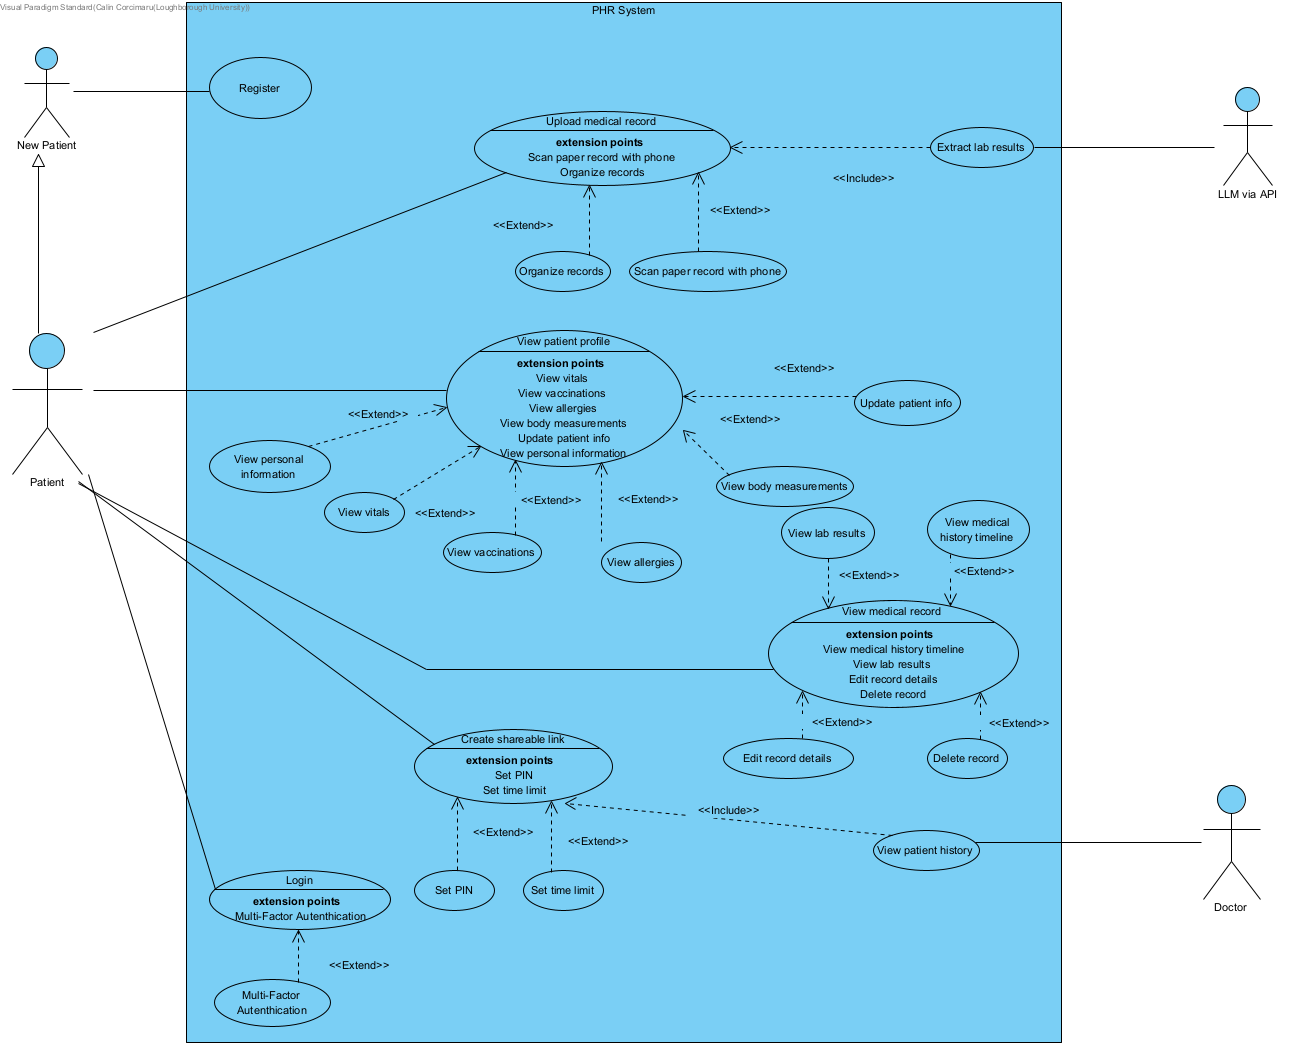
\includegraphics[width=\textwidth,height=0.7\textheight,keepaspectratio]{Use_Case.png}
    \caption{UML Use Case Diagram}
    \label{fig:uml_usecase}
\end{figure}

\FloatBarrier

\subsection{Use Case Specifications}

\subsubsection{Login}
\begin{tabular}{|p{0.2\textwidth}|p{0.7\textwidth}|}
\hline
Description & The Login use case allows the app user to log in to their existing account via their credentials, with an optional use of MFA. \\
\hline
Actors & Patient \\
\hline
Preconditions & Must have an existing account \\
\hline
Steps & 1. User enters user and password \newline
       2. User clicks on the login button \newline
       3. App validates user credentials \newline
       4. Patient enters MFA code if enabled \newline
       5. App logs user in \\
\hline
\end{tabular}

\subsubsection{Register}
\begin{tabular}{|p{0.2\textwidth}|p{0.7\textwidth}|}
\hline
Description & The Register use case allows the app user to create a new account. \\
\hline
Actors & New Patient \\
\hline
Preconditions & No existing account with the email used to register \\
\hline
Steps & 1. User enters user and password \newline
       2. User clicks on the register button \newline
       3. App validates user credentials \newline
       4. App logs user in \newline
       5. App sends verification email \newline
       6. User verifies email \\
\hline
\end{tabular}

\subsubsection{Upload Record}
\begin{tabular}{|p{0.2\textwidth}|p{0.7\textwidth}|}
\hline
Description & The Upload Record use case allows the patient to upload their medical records to the app. \\
\hline
Actors & Patient, LLM \\
\hline
Preconditions & Must be logged in \\
\hline
Steps & 1. User selects file upload (or camera scan) \newline
       2. User selects the record to upload \newline
       3. User clicks on the upload button \newline
       4. App validates the record \newline
       5. User selects the appropriate record type \newline
       6. If record type is lab result, app sends the record to LLM via API for processing into JSON format \newline
       7. App adds the record to the database \newline
       8. App shows confirmation to user \\
\hline
\end{tabular}

\subsubsection{Share Records}
\begin{tabular}{|p{0.2\textwidth}|p{0.7\textwidth}|}
\hline
Description & The Share Records use case allows the patient to share their medical records with doctors. \\
\hline
Actors & Patient, Doctor \\
\hline
Preconditions & Must be logged in and have records uploaded \\
\hline
Steps & 1. User selects option to create a share link \newline
       2. OPTIONAL: User selects the records to share \newline
       3. OPTIONAL: User adds a PIN to the share link \newline
       4. User selects time limit for the share link \newline
       5. App generates the share link \newline
       6. App sends the share link to the doctor via email \newline
       7. App shows confirmation to user \newline
       8. Doctor clicks on the share link \newline
       9. Doctor enters the PIN (if required) \newline
       10. App validates the PIN \newline
       11. App shows the records to the doctor \\
\hline
\end{tabular}

\subsubsection{View Records}
\begin{tabular}{|p{0.2\textwidth}|p{0.7\textwidth}|}
\hline
Description & The View Records use case allows the patient to view and edit their uploaded medical records. \\
\hline
Actors & Patient \\
\hline
Preconditions & Must be logged in and have records uploaded \\
\hline
Steps & 1. App provides a list of records or medical history \newline
       2. User selects record to view from list or medical history \newline
       3. App retrieves the record from the database \newline
       4. App shows the record to the user \newline
       5. OPTIONAL: User can view the record in a graphical format if lab result \newline
       6. OPTIONAL: User edits the record \newline
       7. OPTIONAL: User deletes the record \\
\hline
\end{tabular}

\subsubsection{View Patient Profile}
\begin{tabular}{|p{0.2\textwidth}|p{0.7\textwidth}|}
\hline
Description & The View Patient Profile use case allows the patient to view and edit their profile information, including health information such as allergies, medications, vaccinations and recorded health data like blood pressure, glucose levels, etc. \\
\hline
Actors & Patient \\
\hline
Preconditions & Must be logged in \\
\hline
Steps & 1. User selects the profile section \newline
       2. App retrieves the profile information from the database \newline
       3. App shows the profile information to the user - vaccinations, allergies, medications, health data \newline
       4. OPTIONAL: User edits the profile information \newline
       5. OPTIONAL: User adds new health data \newline
       6. OPTIONAL: User deletes health data \newline
       7. OPTIONAL: User can view health data in a graphical format \\
\hline
\end{tabular}

\FloatBarrier
\clearpage

\subsection{Class Diagram}
\begin{figure}[htbp]
    \centering
    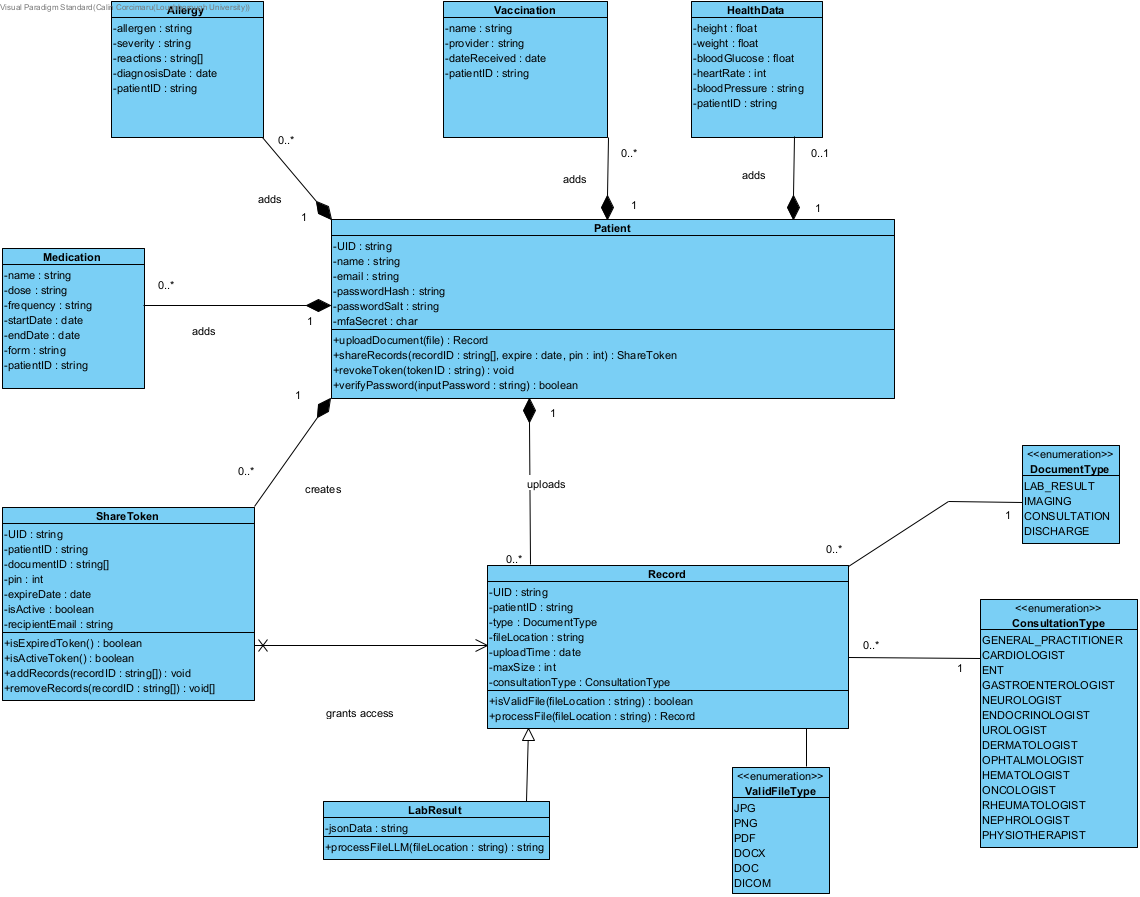
\includegraphics[width=\textwidth,height=0.8\textheight,keepaspectratio]{Class_diagram.png}
    \caption{UML Class Diagram}
    \label{fig:uml_class}
\end{figure}

\FloatBarrier
\clearpage

\subsection{Sequence Diagrams}
\begin{figure}[htbp]
    \centering
    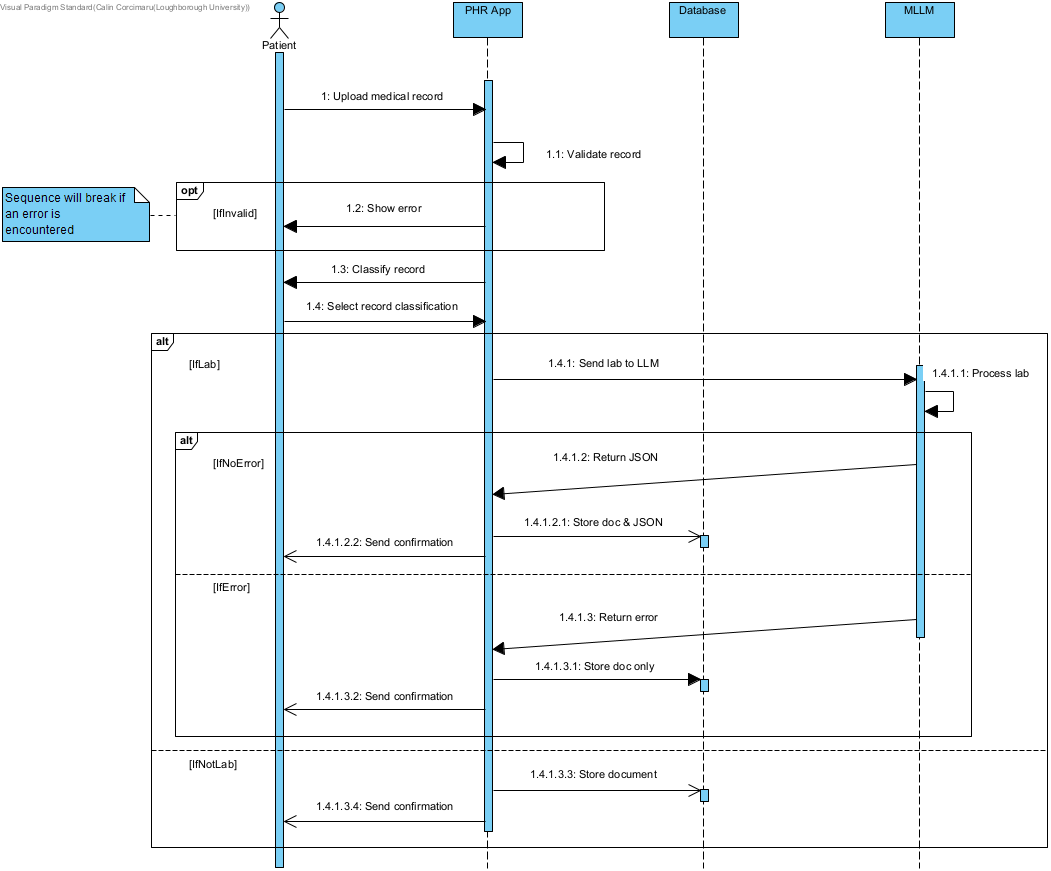
\includegraphics[width=\textwidth,height=0.8\textheight,keepaspectratio]{Sequence_upload.png}
    \caption{UML Sequence Diagram - Upload Record Use Case}
    \label{fig:sequence1}
\end{figure}

\begin{figure}[htbp]
    \centering
    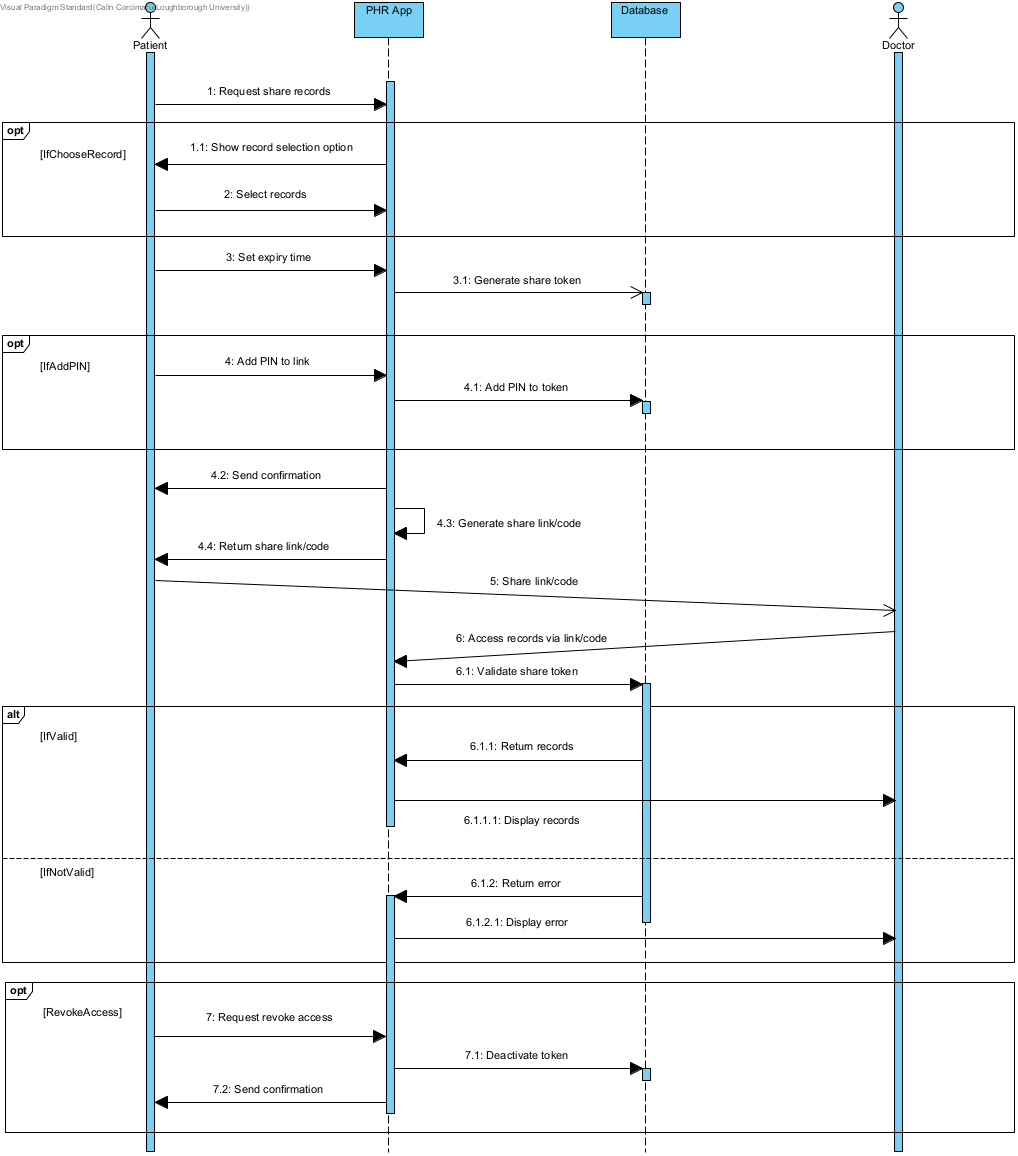
\includegraphics[width=\textwidth,height=0.8\textheight,keepaspectratio]{Sequence_share.png}
    \caption{UML Sequence Diagram - Share Records Use Case}
    \label{fig:sequence2}
\end{figure}

\FloatBarrier

\noindent\begin{minipage}{\textwidth}
    \subsection{Activity Diagrams}
    \begin{center}
        \rotatebox[origin=c]{270}{
            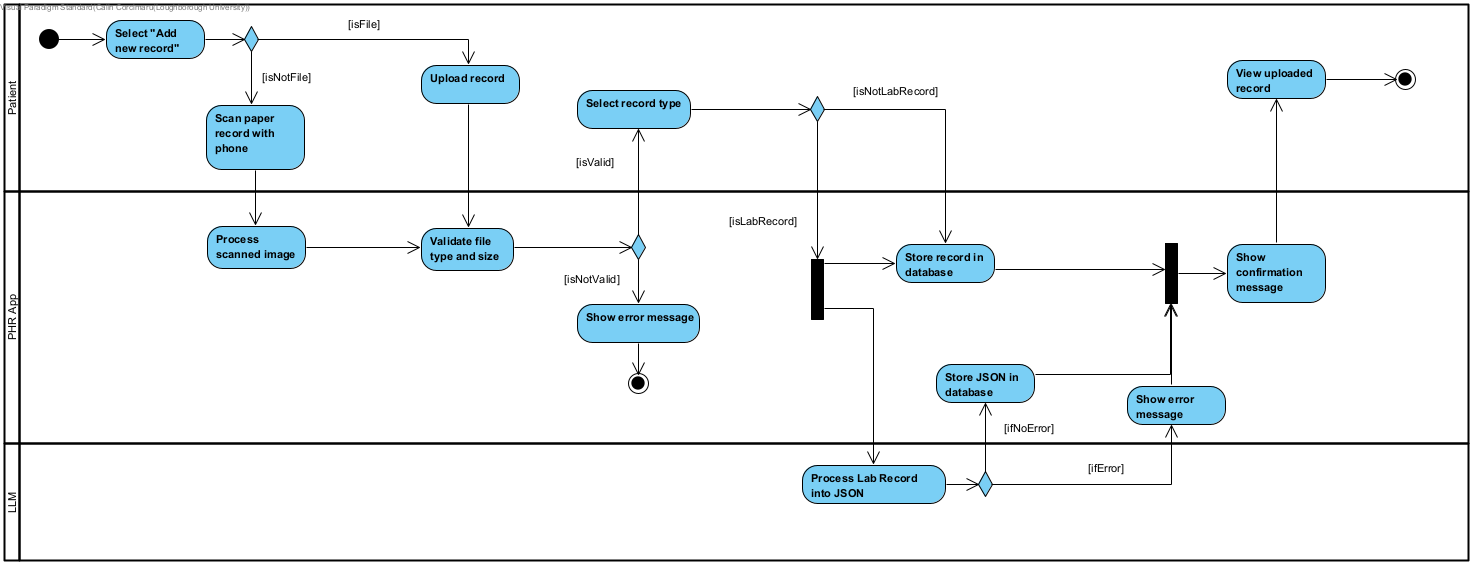
\includegraphics[width=0.9\textheight,keepaspectratio]{Activity_upload.png}
        }
        \captionof{figure}{UML Activity Diagram - Upload Record Use Case}
        \label{fig:activity1}
    \end{center}
\end{minipage}

\noindent\begin{minipage}{\textwidth}
    \begin{center}
        \rotatebox[origin=c]{270}{
            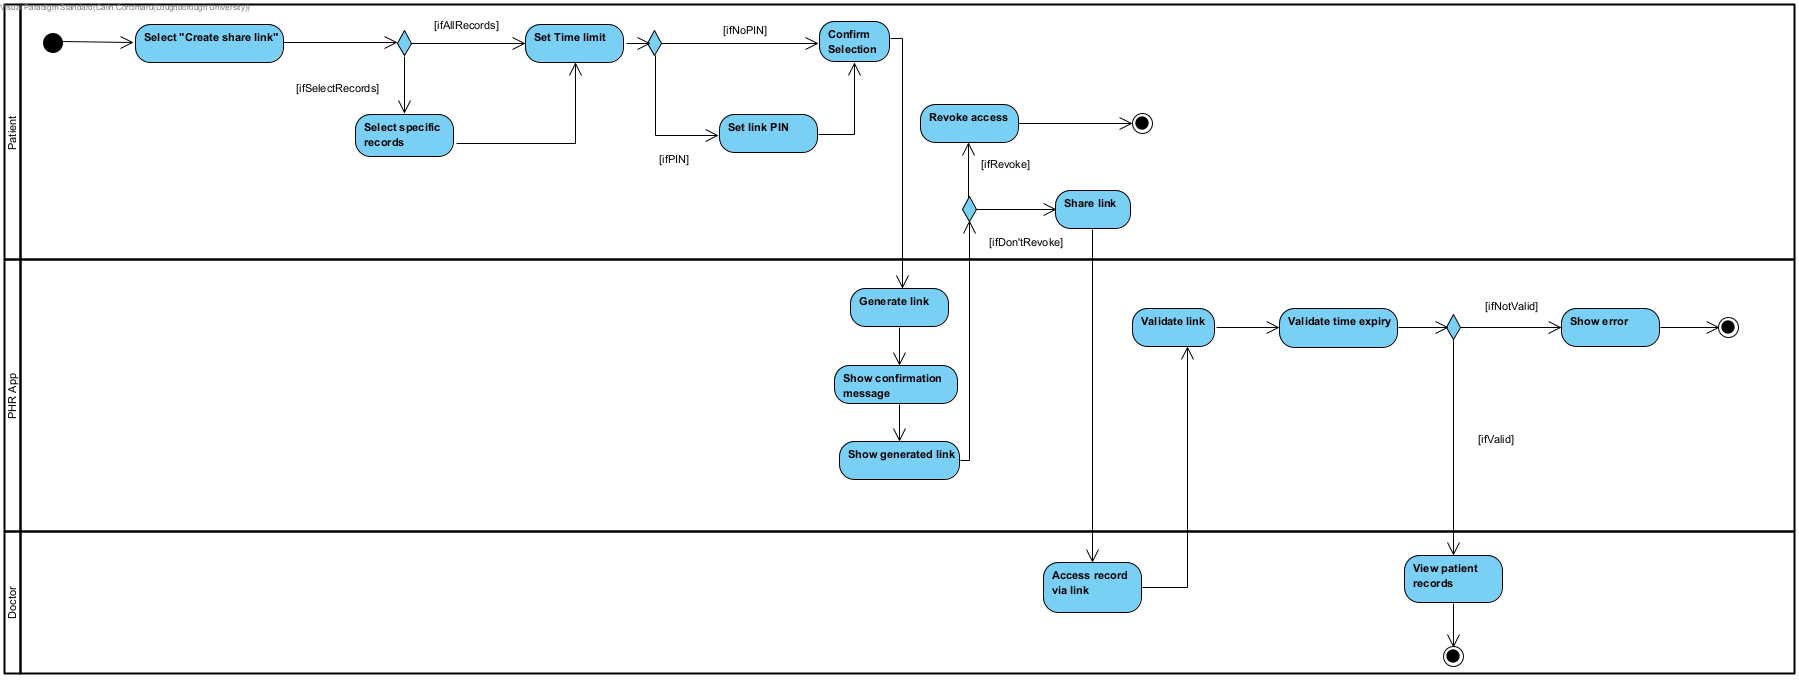
\includegraphics[width=0.9\textheight,keepaspectratio]{Activity_link.png}
        }
        \captionof{figure}{UML Activity Diagram - Share Records Use Case}
        \label{fig:activity2}
    \end{center}
\end{minipage}

\FloatBarrier

\noindent\begin{minipage}{\textwidth}
    \section{Database Design}
    \begin{center}
        \rotatebox[origin=c]{270}{
            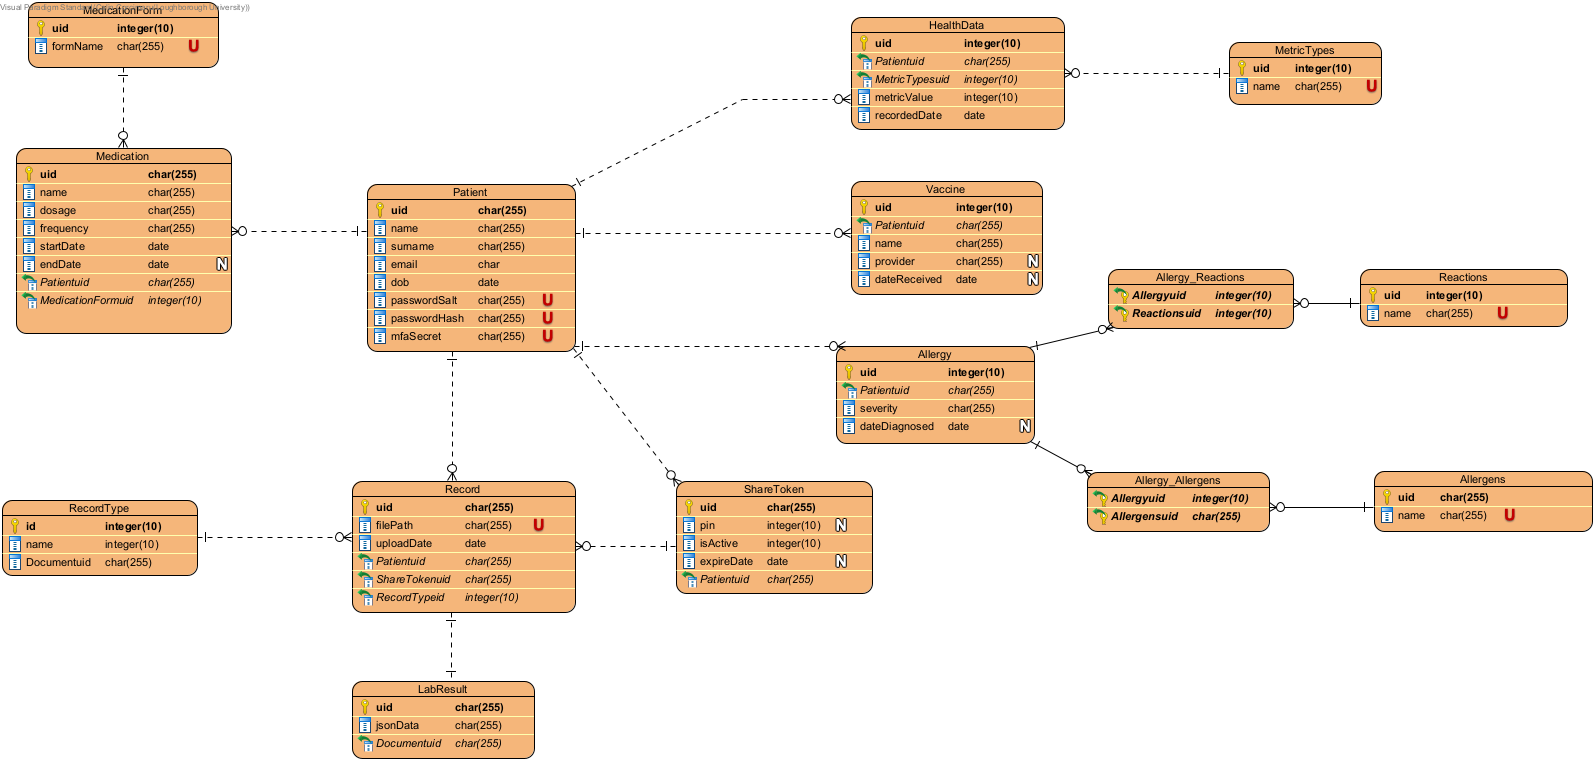
\includegraphics[width=0.9\textheight,keepaspectratio]{ERD.png}
        }
        \captionof{figure}{Entity Relationship Diagram}
        \label{fig:erd}
    \end{center}
\end{minipage}

\FloatBarrier

\section{Wireframes}

\section{Project Tech Stack}

\subsection{Frontend}

\subsection{Backend}

\subsection{Database}

\section{Project Management}

\subsection{Methodology and Tools}

Based on the research above, the student has decided that he will be using a hybrid approach, with Waterfall as the main methodology for planning managing the project. The development part of the project will be done using ScrumBan, so that the student will be able to utilise elements from both frameworks. There are several reasons for this choice:

\begin{enumerate}
    \item The nature of the project - the student is working on a project that has a limited timeframe (about 6-7 months) and is of a smaller scale. 
    \item Documentation requirements - the student is required to document the progress during the project in this report, including the requirements gathered, design considerations and implementation decisions and outcomes. 
    \item Regulatory requirements - the student is required to adhere to the regulations and standards of the healthcare industry, which may require extensive documentation and planning.
    \item Customer involvement - the student will be working closely with the project stakeholder, who will be providing feedback and guidance throughout the project.
    \item Familiarity with both Agile and Waterfall - the student has experience with both Agile (specifically Scrum and Kanban) and Waterfall methodologies, and has worked on projects that have used both approaches.
\end{enumerate}

The student will use Jira Software as their project management tool, which is one of the most popular project management tool for software development projects that supports working with Agile frameworks such as Scrum and Kanban \parencite{atlassian}. The student has experience with Jira Software, having used it in previous projects, and is familiar with its features and capabilities.

\subsection{Project Backlogs}

\subsection{Sprints planning}


% Rename Bibliography to References
%\renewcommand\bibname{References}
\printbibliography[heading=bibintoc, title={References}]

% Include appendix section if needed
%\include{Appendix/Appendix}

\end{document}